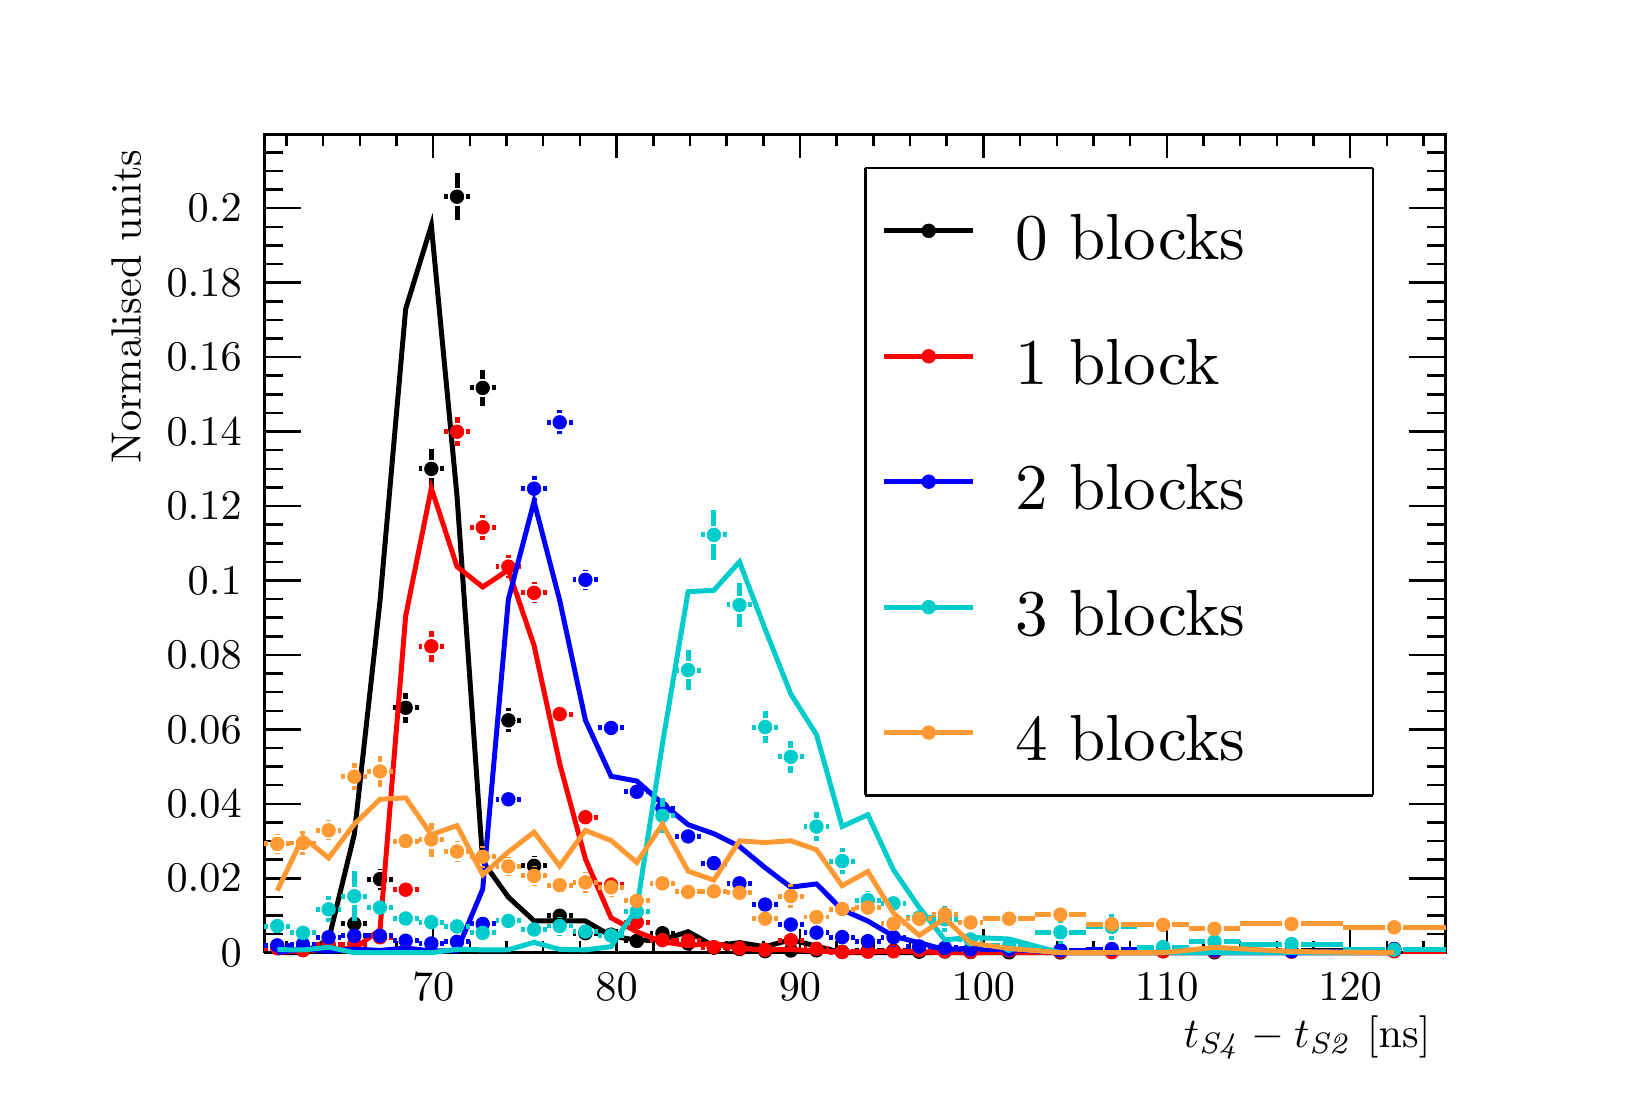
\begin{tikzpicture}
\pgfdeclareplotmark{cross} {
\pgfpathmoveto{\pgfpoint{-0.3\pgfplotmarksize}{\pgfplotmarksize}}
\pgfpathlineto{\pgfpoint{+0.3\pgfplotmarksize}{\pgfplotmarksize}}
\pgfpathlineto{\pgfpoint{+0.3\pgfplotmarksize}{0.3\pgfplotmarksize}}
\pgfpathlineto{\pgfpoint{+1\pgfplotmarksize}{0.3\pgfplotmarksize}}
\pgfpathlineto{\pgfpoint{+1\pgfplotmarksize}{-0.3\pgfplotmarksize}}
\pgfpathlineto{\pgfpoint{+0.3\pgfplotmarksize}{-0.3\pgfplotmarksize}}
\pgfpathlineto{\pgfpoint{+0.3\pgfplotmarksize}{-1.\pgfplotmarksize}}
\pgfpathlineto{\pgfpoint{-0.3\pgfplotmarksize}{-1.\pgfplotmarksize}}
\pgfpathlineto{\pgfpoint{-0.3\pgfplotmarksize}{-0.3\pgfplotmarksize}}
\pgfpathlineto{\pgfpoint{-1.\pgfplotmarksize}{-0.3\pgfplotmarksize}}
\pgfpathlineto{\pgfpoint{-1.\pgfplotmarksize}{0.3\pgfplotmarksize}}
\pgfpathlineto{\pgfpoint{-0.3\pgfplotmarksize}{0.3\pgfplotmarksize}}
\pgfpathclose
\pgfusepathqstroke
}
\pgfdeclareplotmark{cross*} {
\pgfpathmoveto{\pgfpoint{-0.3\pgfplotmarksize}{\pgfplotmarksize}}
\pgfpathlineto{\pgfpoint{+0.3\pgfplotmarksize}{\pgfplotmarksize}}
\pgfpathlineto{\pgfpoint{+0.3\pgfplotmarksize}{0.3\pgfplotmarksize}}
\pgfpathlineto{\pgfpoint{+1\pgfplotmarksize}{0.3\pgfplotmarksize}}
\pgfpathlineto{\pgfpoint{+1\pgfplotmarksize}{-0.3\pgfplotmarksize}}
\pgfpathlineto{\pgfpoint{+0.3\pgfplotmarksize}{-0.3\pgfplotmarksize}}
\pgfpathlineto{\pgfpoint{+0.3\pgfplotmarksize}{-1.\pgfplotmarksize}}
\pgfpathlineto{\pgfpoint{-0.3\pgfplotmarksize}{-1.\pgfplotmarksize}}
\pgfpathlineto{\pgfpoint{-0.3\pgfplotmarksize}{-0.3\pgfplotmarksize}}
\pgfpathlineto{\pgfpoint{-1.\pgfplotmarksize}{-0.3\pgfplotmarksize}}
\pgfpathlineto{\pgfpoint{-1.\pgfplotmarksize}{0.3\pgfplotmarksize}}
\pgfpathlineto{\pgfpoint{-0.3\pgfplotmarksize}{0.3\pgfplotmarksize}}
\pgfpathclose
\pgfusepathqfillstroke
}
\pgfdeclareplotmark{newstar} {
\pgfpathmoveto{\pgfqpoint{0pt}{\pgfplotmarksize}}
\pgfpathlineto{\pgfqpointpolar{44}{0.5\pgfplotmarksize}}
\pgfpathlineto{\pgfqpointpolar{18}{\pgfplotmarksize}}
\pgfpathlineto{\pgfqpointpolar{-20}{0.5\pgfplotmarksize}}
\pgfpathlineto{\pgfqpointpolar{-54}{\pgfplotmarksize}}
\pgfpathlineto{\pgfqpointpolar{-90}{0.5\pgfplotmarksize}}
\pgfpathlineto{\pgfqpointpolar{234}{\pgfplotmarksize}}
\pgfpathlineto{\pgfqpointpolar{198}{0.5\pgfplotmarksize}}
\pgfpathlineto{\pgfqpointpolar{162}{\pgfplotmarksize}}
\pgfpathlineto{\pgfqpointpolar{134}{0.5\pgfplotmarksize}}
\pgfpathclose
\pgfusepathqstroke
}
\pgfdeclareplotmark{newstar*} {
\pgfpathmoveto{\pgfqpoint{0pt}{\pgfplotmarksize}}
\pgfpathlineto{\pgfqpointpolar{44}{0.5\pgfplotmarksize}}
\pgfpathlineto{\pgfqpointpolar{18}{\pgfplotmarksize}}
\pgfpathlineto{\pgfqpointpolar{-20}{0.5\pgfplotmarksize}}
\pgfpathlineto{\pgfqpointpolar{-54}{\pgfplotmarksize}}
\pgfpathlineto{\pgfqpointpolar{-90}{0.5\pgfplotmarksize}}
\pgfpathlineto{\pgfqpointpolar{234}{\pgfplotmarksize}}
\pgfpathlineto{\pgfqpointpolar{198}{0.5\pgfplotmarksize}}
\pgfpathlineto{\pgfqpointpolar{162}{\pgfplotmarksize}}
\pgfpathlineto{\pgfqpointpolar{134}{0.5\pgfplotmarksize}}
\pgfpathclose
\pgfusepathqfillstroke
}
\definecolor{c}{rgb}{1,1,1};
\draw [color=c, fill=c] (0,0) rectangle (20,13.4957);
\draw [color=c, fill=c] (3,1.75444) rectangle (18,12.1461);
\definecolor{c}{rgb}{0,0,0};
\draw [c,line width=0.9] (3,1.75444) -- (3,12.1461) -- (18,12.1461) -- (18,1.75444) -- (3,1.75444);
\definecolor{c}{rgb}{1,1,1};
\draw [color=c, fill=c] (3,1.75444) rectangle (18,12.1461);
\definecolor{c}{rgb}{0,0,0};
\draw [c,line width=0.9] (3,1.75444) -- (3,12.1461) -- (18,12.1461) -- (18,1.75444) -- (3,1.75444);
\draw [c,line width=1.8] (3,1.83114) -- (3.04843,1.83114);
\draw [c,line width=1.8] (3.27766,1.83114) -- (3.32609,1.83114);
\foreach \P in {(3.16304,1.83114)}{\draw[mark options={color=c,fill=c},mark size=2.402402pt,mark=*] plot coordinates {\P};}
\draw [c,line width=1.8] (3.32609,1.82516) -- (3.37452,1.82516);
\draw [c,line width=1.8] (3.60374,1.82516) -- (3.65217,1.82516);
\foreach \P in {(3.48913,1.82516)}{\draw[mark options={color=c,fill=c},mark size=2.402402pt,mark=*] plot coordinates {\P};}
\draw [c,line width=1.8] (3.65217,1.84454) -- (3.7006,1.84454);
\draw [c,line width=1.8] (3.92983,1.84454) -- (3.97826,1.84454);
\foreach \P in {(3.81522,1.84454)}{\draw[mark options={color=c,fill=c},mark size=2.402402pt,mark=*] plot coordinates {\P};}
\draw [c,line width=1.8] (3.97826,2.12085) -- (4.02669,2.12085);
\draw [c,line width=1.8] (4.25592,2.12085) -- (4.30435,2.12085);
\foreach \P in {(4.1413,2.12085)}{\draw[mark options={color=c,fill=c},mark size=2.402402pt,mark=*] plot coordinates {\P};}
\draw [c,line width=1.8] (4.46739,2.55475) -- (4.46739,2.57465);
\draw [c,line width=1.8] (4.46739,2.80387) -- (4.46739,2.82376);
\draw [c,line width=1.8] (4.30435,2.68926) -- (4.35278,2.68926);
\draw [c,line width=1.8] (4.582,2.68926) -- (4.63043,2.68926);
\foreach \P in {(4.46739,2.68926)}{\draw[mark options={color=c,fill=c},mark size=2.402402pt,mark=*] plot coordinates {\P};}
\draw [c,line width=1.8] (4.79348,4.67286) -- (4.79348,4.75114);
\draw [c,line width=1.8] (4.79348,4.98037) -- (4.79348,5.05865);
\draw [c,line width=1.8] (4.63043,4.86575) -- (4.67886,4.86575);
\draw [c,line width=1.8] (4.90809,4.86575) -- (4.95652,4.86575);
\foreach \P in {(4.79348,4.86575)}{\draw[mark options={color=c,fill=c},mark size=2.402402pt,mark=*] plot coordinates {\P};}
\draw [c,line width=1.8] (5.11957,7.64548) -- (5.11957,7.78469);
\draw [c,line width=1.8] (5.11957,8.01391) -- (5.11957,8.15312);
\draw [c,line width=1.8] (4.95652,7.8993) -- (5.00495,7.8993);
\draw [c,line width=1.8] (5.23418,7.8993) -- (5.28261,7.8993);
\foreach \P in {(5.11957,7.8993)}{\draw[mark options={color=c,fill=c},mark size=2.402402pt,mark=*] plot coordinates {\P};}
\draw [c,line width=1.8] (5.44565,11.0614) -- (5.44565,11.2417);
\draw [c,line width=1.8] (5.44565,11.4709) -- (5.44565,11.6513);
\draw [c,line width=1.8] (5.28261,11.3563) -- (5.33104,11.3563);
\draw [c,line width=1.8] (5.56027,11.3563) -- (5.6087,11.3563);
\foreach \P in {(5.44565,11.3563)}{\draw[mark options={color=c,fill=c},mark size=2.402402pt,mark=*] plot coordinates {\P};}
\draw [c,line width=1.8] (5.77174,8.694) -- (5.77174,8.81308);
\draw [c,line width=1.8] (5.77174,9.04231) -- (5.77174,9.1614);
\draw [c,line width=1.8] (5.6087,8.9277) -- (5.65713,8.9277);
\draw [c,line width=1.8] (5.88635,8.9277) -- (5.93478,8.9277);
\foreach \P in {(5.77174,8.9277)}{\draw[mark options={color=c,fill=c},mark size=2.402402pt,mark=*] plot coordinates {\P};}
\draw [c,line width=1.8] (6.09783,4.55419) -- (6.09783,4.59147);
\draw [c,line width=1.8] (6.09783,4.8207) -- (6.09783,4.85798);
\draw [c,line width=1.8] (5.93478,4.70608) -- (5.98321,4.70608);
\draw [c,line width=1.8] (6.21244,4.70608) -- (6.26087,4.70608);
\foreach \P in {(6.09783,4.70608)}{\draw[mark options={color=c,fill=c},mark size=2.402402pt,mark=*] plot coordinates {\P};}
\draw [c,line width=1.8] (6.42391,2.73278) -- (6.42391,2.74337);
\draw [c,line width=1.8] (6.42391,2.9726) -- (6.42391,2.98319);
\draw [c,line width=1.8] (6.26087,2.85799) -- (6.3093,2.85799);
\draw [c,line width=1.8] (6.53853,2.85799) -- (6.58696,2.85799);
\foreach \P in {(6.42391,2.85799)}{\draw[mark options={color=c,fill=c},mark size=2.402402pt,mark=*] plot coordinates {\P};}
\draw [c,line width=1.8] (6.58696,2.22344) -- (6.63539,2.22344);
\draw [c,line width=1.8] (6.86461,2.22344) -- (6.91304,2.22344);
\foreach \P in {(6.75,2.22344)}{\draw[mark options={color=c,fill=c},mark size=2.402402pt,mark=*] plot coordinates {\P};}
\draw [c,line width=1.8] (6.91304,2.00306) -- (6.96147,2.00306);
\draw [c,line width=1.8] (7.1907,2.00306) -- (7.23913,2.00306);
\foreach \P in {(7.07609,2.00306)}{\draw[mark options={color=c,fill=c},mark size=2.402402pt,mark=*] plot coordinates {\P};}
\draw [c,line width=1.8] (7.23913,1.98414) -- (7.28756,1.98414);
\draw [c,line width=1.8] (7.51679,1.98414) -- (7.56522,1.98414);
\foreach \P in {(7.40217,1.98414)}{\draw[mark options={color=c,fill=c},mark size=2.402402pt,mark=*] plot coordinates {\P};}
\draw [c,line width=1.8] (7.56522,1.90433) -- (7.61365,1.90433);
\draw [c,line width=1.8] (7.84287,1.90433) -- (7.8913,1.90433);
\foreach \P in {(7.72826,1.90433)}{\draw[mark options={color=c,fill=c},mark size=2.402402pt,mark=*] plot coordinates {\P};}
\draw [c,line width=1.8] (7.8913,2.00177) -- (7.93973,2.00177);
\draw [c,line width=1.8] (8.16896,2.00177) -- (8.21739,2.00177);
\foreach \P in {(8.05435,2.00177)}{\draw[mark options={color=c,fill=c},mark size=2.402402pt,mark=*] plot coordinates {\P};}
\draw [c,line width=1.8] (8.21739,1.87216) -- (8.26582,1.87216);
\draw [c,line width=1.8] (8.49505,1.87216) -- (8.54348,1.87216);
\foreach \P in {(8.38043,1.87216)}{\draw[mark options={color=c,fill=c},mark size=2.402402pt,mark=*] plot coordinates {\P};}
\draw [c,line width=1.8] (8.54348,1.81906) -- (8.59191,1.81906);
\draw [c,line width=1.8] (8.82113,1.81906) -- (8.86957,1.81906);
\foreach \P in {(8.70652,1.81906)}{\draw[mark options={color=c,fill=c},mark size=2.402402pt,mark=*] plot coordinates {\P};}
\draw [c,line width=1.8] (8.86957,1.80095) -- (8.918,1.80095);
\draw [c,line width=1.8] (9.14722,1.80095) -- (9.19565,1.80095);
\foreach \P in {(9.03261,1.80095)}{\draw[mark options={color=c,fill=c},mark size=2.402402pt,mark=*] plot coordinates {\P};}
\draw [c,line width=1.8] (9.19565,1.77486) -- (9.24408,1.77486);
\draw [c,line width=1.8] (9.47331,1.77486) -- (9.52174,1.77486);
\foreach \P in {(9.3587,1.77486)}{\draw[mark options={color=c,fill=c},mark size=2.402402pt,mark=*] plot coordinates {\P};}
\draw [c,line width=1.8] (9.52174,1.78306) -- (9.57017,1.78306);
\draw [c,line width=1.8] (9.7994,1.78306) -- (9.84783,1.78306);
\foreach \P in {(9.68478,1.78306)}{\draw[mark options={color=c,fill=c},mark size=2.402402pt,mark=*] plot coordinates {\P};}
\draw [c,line width=1.8] (9.84783,1.78487) -- (9.89626,1.78487);
\draw [c,line width=1.8] (10.1255,1.78487) -- (10.1739,1.78487);
\foreach \P in {(10.0109,1.78487)}{\draw[mark options={color=c,fill=c},mark size=2.402402pt,mark=*] plot coordinates {\P};}
\draw [c,line width=1.8] (10.1739,1.76533) -- (10.2223,1.76533);
\draw [c,line width=1.8] (10.4516,1.76533) -- (10.5,1.76533);
\foreach \P in {(10.337,1.76533)}{\draw[mark options={color=c,fill=c},mark size=2.402402pt,mark=*] plot coordinates {\P};}
\draw [c,line width=1.8] (10.5,1.7786) -- (10.5484,1.7786);
\draw [c,line width=1.8] (10.7777,1.7786) -- (10.8261,1.7786);
\foreach \P in {(10.663,1.7786)}{\draw[mark options={color=c,fill=c},mark size=2.402402pt,mark=*] plot coordinates {\P};}
\draw [c,line width=1.8] (10.8261,1.78124) -- (10.8745,1.78124);
\draw [c,line width=1.8] (11.1037,1.78124) -- (11.1522,1.78124);
\foreach \P in {(10.9891,1.78124)}{\draw[mark options={color=c,fill=c},mark size=2.402402pt,mark=*] plot coordinates {\P};}
\draw [c,line width=1.8] (11.1522,1.767) -- (11.2006,1.767);
\draw [c,line width=1.8] (11.4298,1.767) -- (11.4783,1.767);
\foreach \P in {(11.3152,1.767)}{\draw[mark options={color=c,fill=c},mark size=2.402402pt,mark=*] plot coordinates {\P};}
\draw [c,line width=1.8] (11.4783,1.77006) -- (11.5267,1.77006);
\draw [c,line width=1.8] (11.7559,1.77006) -- (11.8043,1.77006);
\foreach \P in {(11.6413,1.77006)}{\draw[mark options={color=c,fill=c},mark size=2.402402pt,mark=*] plot coordinates {\P};}
\draw [c,line width=1.8] (11.8043,1.76448) -- (11.8528,1.76448);
\draw [c,line width=1.8] (12.082,1.76448) -- (12.1304,1.76448);
\foreach \P in {(11.9674,1.76448)}{\draw[mark options={color=c,fill=c},mark size=2.402402pt,mark=*] plot coordinates {\P};}
\draw [c,line width=1.8] (12.1304,1.76013) -- (12.3419,1.76013);
\draw [c,line width=1.8] (12.5711,1.76013) -- (12.7826,1.76013);
\foreach \P in {(12.4565,1.76013)}{\draw[mark options={color=c,fill=c},mark size=2.402402pt,mark=*] plot coordinates {\P};}
\draw [c,line width=1.8] (12.7826,1.75877) -- (12.9941,1.75877);
\draw [c,line width=1.8] (13.2233,1.75877) -- (13.4348,1.75877);
\foreach \P in {(13.1087,1.75877)}{\draw[mark options={color=c,fill=c},mark size=2.402402pt,mark=*] plot coordinates {\P};}
\draw [c,line width=1.8] (13.4348,1.7716) -- (13.6463,1.7716);
\draw [c,line width=1.8] (13.8755,1.7716) -- (14.087,1.7716);
\foreach \P in {(13.7609,1.7716)}{\draw[mark options={color=c,fill=c},mark size=2.402402pt,mark=*] plot coordinates {\P};}
\draw [c,line width=1.8] (14.087,1.77325) -- (14.2984,1.77325);
\draw [c,line width=1.8] (14.5277,1.77325) -- (14.7391,1.77325);
\foreach \P in {(14.413,1.77325)}{\draw[mark options={color=c,fill=c},mark size=2.402402pt,mark=*] plot coordinates {\P};}
\draw [c,line width=1.8] (14.7391,1.76012) -- (14.9506,1.76012);
\draw [c,line width=1.8] (15.1798,1.76012) -- (15.3913,1.76012);
\foreach \P in {(15.0652,1.76012)}{\draw[mark options={color=c,fill=c},mark size=2.402402pt,mark=*] plot coordinates {\P};}
\draw [c,line width=1.8] (15.3913,1.77863) -- (15.9289,1.77863);
\draw [c,line width=1.8] (16.1581,1.77863) -- (16.6957,1.77863);
\foreach \P in {(16.0435,1.77863)}{\draw[mark options={color=c,fill=c},mark size=2.402402pt,mark=*] plot coordinates {\P};}
\draw [c,line width=1.8] (16.6957,1.80192) -- (17.2332,1.80192);
\draw [c,line width=1.8] (17.4624,1.80192) -- (18,1.80192);
\foreach \P in {(17.3478,1.80192)}{\draw[mark options={color=c,fill=c},mark size=2.402402pt,mark=*] plot coordinates {\P};}
\draw [c,line width=0.9] (3,1.75444) -- (18,1.75444);
\draw [c,line width=0.9] (5.14286,2.05809) -- (5.14286,1.75444);
\draw [c,line width=0.9] (5.6087,1.90627) -- (5.6087,1.75444);
\draw [c,line width=0.9] (6.07453,1.90627) -- (6.07453,1.75444);
\draw [c,line width=0.9] (6.54037,1.90627) -- (6.54037,1.75444);
\draw [c,line width=0.9] (7.00621,1.90627) -- (7.00621,1.75444);
\draw [c,line width=0.9] (7.47205,2.05809) -- (7.47205,1.75444);
\draw [c,line width=0.9] (7.93789,1.90627) -- (7.93789,1.75444);
\draw [c,line width=0.9] (8.40373,1.90627) -- (8.40373,1.75444);
\draw [c,line width=0.9] (8.86957,1.90627) -- (8.86957,1.75444);
\draw [c,line width=0.9] (9.3354,1.90627) -- (9.3354,1.75444);
\draw [c,line width=0.9] (9.80124,2.05809) -- (9.80124,1.75444);
\draw [c,line width=0.9] (10.2671,1.90627) -- (10.2671,1.75444);
\draw [c,line width=0.9] (10.7329,1.90627) -- (10.7329,1.75444);
\draw [c,line width=0.9] (11.1988,1.90627) -- (11.1988,1.75444);
\draw [c,line width=0.9] (11.6646,1.90627) -- (11.6646,1.75444);
\draw [c,line width=0.9] (12.1304,2.05809) -- (12.1304,1.75444);
\draw [c,line width=0.9] (12.5963,1.90627) -- (12.5963,1.75444);
\draw [c,line width=0.9] (13.0621,1.90627) -- (13.0621,1.75444);
\draw [c,line width=0.9] (13.528,1.90627) -- (13.528,1.75444);
\draw [c,line width=0.9] (13.9938,1.90627) -- (13.9938,1.75444);
\draw [c,line width=0.9] (14.4596,2.05809) -- (14.4596,1.75444);
\draw [c,line width=0.9] (14.9255,1.90627) -- (14.9255,1.75444);
\draw [c,line width=0.9] (15.3913,1.90627) -- (15.3913,1.75444);
\draw [c,line width=0.9] (15.8571,1.90627) -- (15.8571,1.75444);
\draw [c,line width=0.9] (16.323,1.90627) -- (16.323,1.75444);
\draw [c,line width=0.9] (16.7888,2.05809) -- (16.7888,1.75444);
\draw [c,line width=0.9] (5.14286,2.05809) -- (5.14286,1.75444);
\draw [c,line width=0.9] (4.67702,1.90627) -- (4.67702,1.75444);
\draw [c,line width=0.9] (4.21118,1.90627) -- (4.21118,1.75444);
\draw [c,line width=0.9] (3.74534,1.90627) -- (3.74534,1.75444);
\draw [c,line width=0.9] (3.2795,1.90627) -- (3.2795,1.75444);
\draw [c,line width=0.9] (16.7888,2.05809) -- (16.7888,1.75444);
\draw [c,line width=0.9] (17.2547,1.90627) -- (17.2547,1.75444);
\draw [c,line width=0.9] (17.7205,1.90627) -- (17.7205,1.75444);
\draw [anchor=base] (5.14286,1.14713) node[scale=1.52731, color=c, rotate=0]{70};
\draw [anchor=base] (7.47205,1.14713) node[scale=1.52731, color=c, rotate=0]{80};
\draw [anchor=base] (9.80124,1.14713) node[scale=1.52731, color=c, rotate=0]{90};
\draw [anchor=base] (12.1304,1.14713) node[scale=1.52731, color=c, rotate=0]{100};
\draw [anchor=base] (14.4596,1.14713) node[scale=1.52731, color=c, rotate=0]{110};
\draw [anchor=base] (16.7888,1.14713) node[scale=1.52731, color=c, rotate=0]{120};
\draw [anchor= east] (18,0.674785) node[scale=1.52731, color=c, rotate=0]{$t_{\mathit{S4}} - t_{\mathit{S2}}$ [ns]};
\draw [c,line width=0.9] (3,12.1461) -- (18,12.1461);
\draw [c,line width=0.9] (5.14286,11.8425) -- (5.14286,12.1461);
\draw [c,line width=0.9] (5.6087,11.9943) -- (5.6087,12.1461);
\draw [c,line width=0.9] (6.07453,11.9943) -- (6.07453,12.1461);
\draw [c,line width=0.9] (6.54037,11.9943) -- (6.54037,12.1461);
\draw [c,line width=0.9] (7.00621,11.9943) -- (7.00621,12.1461);
\draw [c,line width=0.9] (7.47205,11.8425) -- (7.47205,12.1461);
\draw [c,line width=0.9] (7.93789,11.9943) -- (7.93789,12.1461);
\draw [c,line width=0.9] (8.40373,11.9943) -- (8.40373,12.1461);
\draw [c,line width=0.9] (8.86957,11.9943) -- (8.86957,12.1461);
\draw [c,line width=0.9] (9.3354,11.9943) -- (9.3354,12.1461);
\draw [c,line width=0.9] (9.80124,11.8425) -- (9.80124,12.1461);
\draw [c,line width=0.9] (10.2671,11.9943) -- (10.2671,12.1461);
\draw [c,line width=0.9] (10.7329,11.9943) -- (10.7329,12.1461);
\draw [c,line width=0.9] (11.1988,11.9943) -- (11.1988,12.1461);
\draw [c,line width=0.9] (11.6646,11.9943) -- (11.6646,12.1461);
\draw [c,line width=0.9] (12.1304,11.8425) -- (12.1304,12.1461);
\draw [c,line width=0.9] (12.5963,11.9943) -- (12.5963,12.1461);
\draw [c,line width=0.9] (13.0621,11.9943) -- (13.0621,12.1461);
\draw [c,line width=0.9] (13.528,11.9943) -- (13.528,12.1461);
\draw [c,line width=0.9] (13.9938,11.9943) -- (13.9938,12.1461);
\draw [c,line width=0.9] (14.4596,11.8425) -- (14.4596,12.1461);
\draw [c,line width=0.9] (14.9255,11.9943) -- (14.9255,12.1461);
\draw [c,line width=0.9] (15.3913,11.9943) -- (15.3913,12.1461);
\draw [c,line width=0.9] (15.8571,11.9943) -- (15.8571,12.1461);
\draw [c,line width=0.9] (16.323,11.9943) -- (16.323,12.1461);
\draw [c,line width=0.9] (16.7888,11.8425) -- (16.7888,12.1461);
\draw [c,line width=0.9] (5.14286,11.8425) -- (5.14286,12.1461);
\draw [c,line width=0.9] (4.67702,11.9943) -- (4.67702,12.1461);
\draw [c,line width=0.9] (4.21118,11.9943) -- (4.21118,12.1461);
\draw [c,line width=0.9] (3.74534,11.9943) -- (3.74534,12.1461);
\draw [c,line width=0.9] (3.2795,11.9943) -- (3.2795,12.1461);
\draw [c,line width=0.9] (16.7888,11.8425) -- (16.7888,12.1461);
\draw [c,line width=0.9] (17.2547,11.9943) -- (17.2547,12.1461);
\draw [c,line width=0.9] (17.7205,11.9943) -- (17.7205,12.1461);
\draw [c,line width=0.9] (3,1.75444) -- (3,12.1461);
\draw [c,line width=0.9] (3.462,1.75444) -- (3,1.75444);
\draw [c,line width=0.9] (3.231,1.99082) -- (3,1.99082);
\draw [c,line width=0.9] (3.231,2.2272) -- (3,2.2272);
\draw [c,line width=0.9] (3.231,2.46357) -- (3,2.46357);
\draw [c,line width=0.9] (3.462,2.69995) -- (3,2.69995);
\draw [c,line width=0.9] (3.231,2.93633) -- (3,2.93633);
\draw [c,line width=0.9] (3.231,3.1727) -- (3,3.1727);
\draw [c,line width=0.9] (3.231,3.40908) -- (3,3.40908);
\draw [c,line width=0.9] (3.462,3.64546) -- (3,3.64546);
\draw [c,line width=0.9] (3.231,3.88184) -- (3,3.88184);
\draw [c,line width=0.9] (3.231,4.11821) -- (3,4.11821);
\draw [c,line width=0.9] (3.231,4.35459) -- (3,4.35459);
\draw [c,line width=0.9] (3.462,4.59097) -- (3,4.59097);
\draw [c,line width=0.9] (3.231,4.82734) -- (3,4.82734);
\draw [c,line width=0.9] (3.231,5.06372) -- (3,5.06372);
\draw [c,line width=0.9] (3.231,5.3001) -- (3,5.3001);
\draw [c,line width=0.9] (3.462,5.53648) -- (3,5.53648);
\draw [c,line width=0.9] (3.231,5.77285) -- (3,5.77285);
\draw [c,line width=0.9] (3.231,6.00923) -- (3,6.00923);
\draw [c,line width=0.9] (3.231,6.24561) -- (3,6.24561);
\draw [c,line width=0.9] (3.462,6.48199) -- (3,6.48199);
\draw [c,line width=0.9] (3.231,6.71836) -- (3,6.71836);
\draw [c,line width=0.9] (3.231,6.95474) -- (3,6.95474);
\draw [c,line width=0.9] (3.231,7.19112) -- (3,7.19112);
\draw [c,line width=0.9] (3.462,7.42749) -- (3,7.42749);
\draw [c,line width=0.9] (3.231,7.66387) -- (3,7.66387);
\draw [c,line width=0.9] (3.231,7.90025) -- (3,7.90025);
\draw [c,line width=0.9] (3.231,8.13663) -- (3,8.13663);
\draw [c,line width=0.9] (3.462,8.373) -- (3,8.373);
\draw [c,line width=0.9] (3.231,8.60938) -- (3,8.60938);
\draw [c,line width=0.9] (3.231,8.84576) -- (3,8.84576);
\draw [c,line width=0.9] (3.231,9.08213) -- (3,9.08213);
\draw [c,line width=0.9] (3.462,9.31851) -- (3,9.31851);
\draw [c,line width=0.9] (3.231,9.55489) -- (3,9.55489);
\draw [c,line width=0.9] (3.231,9.79127) -- (3,9.79127);
\draw [c,line width=0.9] (3.231,10.0276) -- (3,10.0276);
\draw [c,line width=0.9] (3.462,10.264) -- (3,10.264);
\draw [c,line width=0.9] (3.231,10.5004) -- (3,10.5004);
\draw [c,line width=0.9] (3.231,10.7368) -- (3,10.7368);
\draw [c,line width=0.9] (3.231,10.9732) -- (3,10.9732);
\draw [c,line width=0.9] (3.462,11.2095) -- (3,11.2095);
\draw [c,line width=0.9] (3.462,11.2095) -- (3,11.2095);
\draw [c,line width=0.9] (3.231,11.4459) -- (3,11.4459);
\draw [c,line width=0.9] (3.231,11.6823) -- (3,11.6823);
\draw [c,line width=0.9] (3.231,11.9187) -- (3,11.9187);
\draw [anchor= east] (2.9,1.75444) node[scale=1.52731, color=c, rotate=0]{0};
\draw [anchor= east] (2.9,2.69995) node[scale=1.52731, color=c, rotate=0]{0.02};
\draw [anchor= east] (2.9,3.64546) node[scale=1.52731, color=c, rotate=0]{0.04};
\draw [anchor= east] (2.9,4.59097) node[scale=1.52731, color=c, rotate=0]{0.06};
\draw [anchor= east] (2.9,5.53648) node[scale=1.52731, color=c, rotate=0]{0.08};
\draw [anchor= east] (2.9,6.48199) node[scale=1.52731, color=c, rotate=0]{0.1};
\draw [anchor= east] (2.9,7.42749) node[scale=1.52731, color=c, rotate=0]{0.12};
\draw [anchor= east] (2.9,8.373) node[scale=1.52731, color=c, rotate=0]{0.14};
\draw [anchor= east] (2.9,9.31851) node[scale=1.52731, color=c, rotate=0]{0.16};
\draw [anchor= east] (2.9,10.264) node[scale=1.52731, color=c, rotate=0]{0.18};
\draw [anchor= east] (2.9,11.2095) node[scale=1.52731, color=c, rotate=0]{0.2};
\draw [anchor= east] (1.24,12.1461) node[scale=1.52731, color=c, rotate=90]{Normalised units};
\draw [c,line width=0.9] (18,1.75444) -- (18,12.1461);
\draw [c,line width=0.9] (17.538,1.75444) -- (18,1.75444);
\draw [c,line width=0.9] (17.769,1.99082) -- (18,1.99082);
\draw [c,line width=0.9] (17.769,2.2272) -- (18,2.2272);
\draw [c,line width=0.9] (17.769,2.46357) -- (18,2.46357);
\draw [c,line width=0.9] (17.538,2.69995) -- (18,2.69995);
\draw [c,line width=0.9] (17.769,2.93633) -- (18,2.93633);
\draw [c,line width=0.9] (17.769,3.1727) -- (18,3.1727);
\draw [c,line width=0.9] (17.769,3.40908) -- (18,3.40908);
\draw [c,line width=0.9] (17.538,3.64546) -- (18,3.64546);
\draw [c,line width=0.9] (17.769,3.88184) -- (18,3.88184);
\draw [c,line width=0.9] (17.769,4.11821) -- (18,4.11821);
\draw [c,line width=0.9] (17.769,4.35459) -- (18,4.35459);
\draw [c,line width=0.9] (17.538,4.59097) -- (18,4.59097);
\draw [c,line width=0.9] (17.769,4.82734) -- (18,4.82734);
\draw [c,line width=0.9] (17.769,5.06372) -- (18,5.06372);
\draw [c,line width=0.9] (17.769,5.3001) -- (18,5.3001);
\draw [c,line width=0.9] (17.538,5.53648) -- (18,5.53648);
\draw [c,line width=0.9] (17.769,5.77285) -- (18,5.77285);
\draw [c,line width=0.9] (17.769,6.00923) -- (18,6.00923);
\draw [c,line width=0.9] (17.769,6.24561) -- (18,6.24561);
\draw [c,line width=0.9] (17.538,6.48199) -- (18,6.48199);
\draw [c,line width=0.9] (17.769,6.71836) -- (18,6.71836);
\draw [c,line width=0.9] (17.769,6.95474) -- (18,6.95474);
\draw [c,line width=0.9] (17.769,7.19112) -- (18,7.19112);
\draw [c,line width=0.9] (17.538,7.42749) -- (18,7.42749);
\draw [c,line width=0.9] (17.769,7.66387) -- (18,7.66387);
\draw [c,line width=0.9] (17.769,7.90025) -- (18,7.90025);
\draw [c,line width=0.9] (17.769,8.13663) -- (18,8.13663);
\draw [c,line width=0.9] (17.538,8.373) -- (18,8.373);
\draw [c,line width=0.9] (17.769,8.60938) -- (18,8.60938);
\draw [c,line width=0.9] (17.769,8.84576) -- (18,8.84576);
\draw [c,line width=0.9] (17.769,9.08213) -- (18,9.08213);
\draw [c,line width=0.9] (17.538,9.31851) -- (18,9.31851);
\draw [c,line width=0.9] (17.769,9.55489) -- (18,9.55489);
\draw [c,line width=0.9] (17.769,9.79127) -- (18,9.79127);
\draw [c,line width=0.9] (17.769,10.0276) -- (18,10.0276);
\draw [c,line width=0.9] (17.538,10.264) -- (18,10.264);
\draw [c,line width=0.9] (17.769,10.5004) -- (18,10.5004);
\draw [c,line width=0.9] (17.769,10.7368) -- (18,10.7368);
\draw [c,line width=0.9] (17.769,10.9732) -- (18,10.9732);
\draw [c,line width=0.9] (17.538,11.2095) -- (18,11.2095);
\draw [c,line width=0.9] (17.538,11.2095) -- (18,11.2095);
\draw [c,line width=0.9] (17.769,11.4459) -- (18,11.4459);
\draw [c,line width=0.9] (17.769,11.6823) -- (18,11.6823);
\draw [c,line width=0.9] (17.769,11.9187) -- (18,11.9187);
\draw [c,line width=1.8] (3.16304,1.75444) -- (3.48913,1.75444) -- (3.81522,1.91963) -- (4.1413,3.2586) -- (4.46739,6.21923) -- (4.79348,9.93097) -- (5.11957,10.9903) -- (5.44565,7.5521) -- (5.77174,2.91629) -- (6.09783,2.46021) -- (6.42391,2.16031)
 -- (6.75,2.15888) -- (7.07609,2.1576) -- (7.40217,1.96821) -- (7.72826,1.91351) -- (8.05435,1.91827) -- (8.38043,2.02123) -- (8.70652,1.84056) -- (9.03261,1.88256) -- (9.3587,1.83017) -- (9.68478,1.92059) -- (10.0109,1.83781) -- (10.337,1.75444) --
 (10.663,1.75444) -- (10.9891,1.75444) -- (11.3152,1.75444) -- (11.6413,1.75444) -- (11.9674,1.75444) -- (12.4565,1.75444) -- (13.1087,1.75444) -- (13.7609,1.75444) -- (14.413,1.75444) -- (15.0652,1.75444) -- (16.0435,1.75444) -- (17.3478,1.75444);
\definecolor{c}{rgb}{1,0,0};
\draw [c,line width=1.8] (3,1.81211) -- (3.04843,1.81211);
\draw [c,line width=1.8] (3.27766,1.81211) -- (3.32609,1.81211);
\foreach \P in {(3.16304,1.81211)}{\draw[mark options={color=c,fill=c},mark size=2.402402pt,mark=*] plot coordinates {\P};}
\draw [c,line width=1.8] (3.32609,1.78648) -- (3.37452,1.78648);
\draw [c,line width=1.8] (3.60374,1.78648) -- (3.65217,1.78648);
\foreach \P in {(3.48913,1.78648)}{\draw[mark options={color=c,fill=c},mark size=2.402402pt,mark=*] plot coordinates {\P};}
\draw [c,line width=1.8] (3.65217,1.86159) -- (3.7006,1.86159);
\draw [c,line width=1.8] (3.92983,1.86159) -- (3.97826,1.86159);
\foreach \P in {(3.81522,1.86159)}{\draw[mark options={color=c,fill=c},mark size=2.402402pt,mark=*] plot coordinates {\P};}
\draw [c,line width=1.8] (3.97826,1.86397) -- (4.02669,1.86397);
\draw [c,line width=1.8] (4.25592,1.86397) -- (4.30435,1.86397);
\foreach \P in {(4.1413,1.86397)}{\draw[mark options={color=c,fill=c},mark size=2.402402pt,mark=*] plot coordinates {\P};}
\draw [c,line width=1.8] (4.30435,1.95008) -- (4.35278,1.95008);
\draw [c,line width=1.8] (4.582,1.95008) -- (4.63043,1.95008);
\foreach \P in {(4.46739,1.95008)}{\draw[mark options={color=c,fill=c},mark size=2.402402pt,mark=*] plot coordinates {\P};}
\draw [c,line width=1.8] (4.63043,2.55497) -- (4.67886,2.55497);
\draw [c,line width=1.8] (4.90809,2.55497) -- (4.95652,2.55497);
\foreach \P in {(4.79348,2.55497)}{\draw[mark options={color=c,fill=c},mark size=2.402402pt,mark=*] plot coordinates {\P};}
\draw [c,line width=1.8] (5.11957,5.44535) -- (5.11957,5.53144);
\draw [c,line width=1.8] (5.11957,5.76067) -- (5.11957,5.84676);
\draw [c,line width=1.8] (4.95652,5.64606) -- (5.00495,5.64606);
\draw [c,line width=1.8] (5.23418,5.64606) -- (5.28261,5.64606);
\foreach \P in {(5.11957,5.64606)}{\draw[mark options={color=c,fill=c},mark size=2.402402pt,mark=*] plot coordinates {\P};}
\draw [c,line width=1.8] (5.44565,8.18679) -- (5.44565,8.25649);
\draw [c,line width=1.8] (5.44565,8.48571) -- (5.44565,8.55541);
\draw [c,line width=1.8] (5.28261,8.3711) -- (5.33104,8.3711);
\draw [c,line width=1.8] (5.56027,8.3711) -- (5.6087,8.3711);
\foreach \P in {(5.44565,8.3711)}{\draw[mark options={color=c,fill=c},mark size=2.402402pt,mark=*] plot coordinates {\P};}
\draw [c,line width=1.8] (5.77174,6.99625) -- (5.77174,7.04232);
\draw [c,line width=1.8] (5.77174,7.27155) -- (5.77174,7.31762);
\draw [c,line width=1.8] (5.6087,7.15694) -- (5.65713,7.15694);
\draw [c,line width=1.8] (5.88635,7.15694) -- (5.93478,7.15694);
\foreach \P in {(5.77174,7.15694)}{\draw[mark options={color=c,fill=c},mark size=2.402402pt,mark=*] plot coordinates {\P};}
\draw [c,line width=1.8] (6.09783,6.51144) -- (6.09783,6.54373);
\draw [c,line width=1.8] (6.09783,6.77295) -- (6.09783,6.80523);
\draw [c,line width=1.8] (5.93478,6.65834) -- (5.98321,6.65834);
\draw [c,line width=1.8] (6.21244,6.65834) -- (6.26087,6.65834);
\foreach \P in {(6.09783,6.65834)}{\draw[mark options={color=c,fill=c},mark size=2.402402pt,mark=*] plot coordinates {\P};}
\draw [c,line width=1.8] (6.42391,6.19165) -- (6.42391,6.21023);
\draw [c,line width=1.8] (6.42391,6.43946) -- (6.42391,6.45803);
\draw [c,line width=1.8] (6.26087,6.32484) -- (6.3093,6.32484);
\draw [c,line width=1.8] (6.53853,6.32484) -- (6.58696,6.32484);
\foreach \P in {(6.42391,6.32484)}{\draw[mark options={color=c,fill=c},mark size=2.402402pt,mark=*] plot coordinates {\P};}
\draw [c,line width=1.8] (6.58696,4.78522) -- (6.63539,4.78522);
\draw [c,line width=1.8] (6.86461,4.78522) -- (6.91304,4.78522);
\foreach \P in {(6.75,4.78522)}{\draw[mark options={color=c,fill=c},mark size=2.402402pt,mark=*] plot coordinates {\P};}
\draw [c,line width=1.8] (6.91304,3.47547) -- (6.96147,3.47547);
\draw [c,line width=1.8] (7.1907,3.47547) -- (7.23913,3.47547);
\foreach \P in {(7.07609,3.47547)}{\draw[mark options={color=c,fill=c},mark size=2.402402pt,mark=*] plot coordinates {\P};}
\draw [c,line width=1.8] (7.23913,2.61559) -- (7.28756,2.61559);
\draw [c,line width=1.8] (7.51679,2.61559) -- (7.56522,2.61559);
\foreach \P in {(7.40217,2.61559)}{\draw[mark options={color=c,fill=c},mark size=2.402402pt,mark=*] plot coordinates {\P};}
\draw [c,line width=1.8] (7.56522,2.14104) -- (7.61365,2.14104);
\draw [c,line width=1.8] (7.84287,2.14104) -- (7.8913,2.14104);
\foreach \P in {(7.72826,2.14104)}{\draw[mark options={color=c,fill=c},mark size=2.402402pt,mark=*] plot coordinates {\P};}
\draw [c,line width=1.8] (7.8913,1.91483) -- (7.93973,1.91483);
\draw [c,line width=1.8] (8.16896,1.91483) -- (8.21739,1.91483);
\foreach \P in {(8.05435,1.91483)}{\draw[mark options={color=c,fill=c},mark size=2.402402pt,mark=*] plot coordinates {\P};}
\draw [c,line width=1.8] (8.21739,1.90786) -- (8.26582,1.90786);
\draw [c,line width=1.8] (8.49505,1.90786) -- (8.54348,1.90786);
\foreach \P in {(8.38043,1.90786)}{\draw[mark options={color=c,fill=c},mark size=2.402402pt,mark=*] plot coordinates {\P};}
\draw [c,line width=1.8] (8.54348,1.82528) -- (8.59191,1.82528);
\draw [c,line width=1.8] (8.82113,1.82528) -- (8.86957,1.82528);
\foreach \P in {(8.70652,1.82528)}{\draw[mark options={color=c,fill=c},mark size=2.402402pt,mark=*] plot coordinates {\P};}
\draw [c,line width=1.8] (8.86957,1.81201) -- (8.918,1.81201);
\draw [c,line width=1.8] (9.14722,1.81201) -- (9.19565,1.81201);
\foreach \P in {(9.03261,1.81201)}{\draw[mark options={color=c,fill=c},mark size=2.402402pt,mark=*] plot coordinates {\P};}
\draw [c,line width=1.8] (9.19565,1.79221) -- (9.24408,1.79221);
\draw [c,line width=1.8] (9.47331,1.79221) -- (9.52174,1.79221);
\foreach \P in {(9.3587,1.79221)}{\draw[mark options={color=c,fill=c},mark size=2.402402pt,mark=*] plot coordinates {\P};}
\draw [c,line width=1.8] (9.52174,1.91331) -- (9.57017,1.91331);
\draw [c,line width=1.8] (9.7994,1.91331) -- (9.84783,1.91331);
\foreach \P in {(9.68478,1.91331)}{\draw[mark options={color=c,fill=c},mark size=2.402402pt,mark=*] plot coordinates {\P};}
\draw [c,line width=1.8] (9.84783,1.80433) -- (9.89626,1.80433);
\draw [c,line width=1.8] (10.1255,1.80433) -- (10.1739,1.80433);
\foreach \P in {(10.0109,1.80433)}{\draw[mark options={color=c,fill=c},mark size=2.402402pt,mark=*] plot coordinates {\P};}
\draw [c,line width=1.8] (10.1739,1.76343) -- (10.2223,1.76343);
\draw [c,line width=1.8] (10.4516,1.76343) -- (10.5,1.76343);
\foreach \P in {(10.337,1.76343)}{\draw[mark options={color=c,fill=c},mark size=2.402402pt,mark=*] plot coordinates {\P};}
\draw [c,line width=1.8] (10.5,1.76754) -- (10.5484,1.76754);
\draw [c,line width=1.8] (10.7777,1.76754) -- (10.8261,1.76754);
\foreach \P in {(10.663,1.76754)}{\draw[mark options={color=c,fill=c},mark size=2.402402pt,mark=*] plot coordinates {\P};}
\draw [c,line width=1.8] (10.8261,1.77221) -- (10.8745,1.77221);
\draw [c,line width=1.8] (11.1037,1.77221) -- (11.1522,1.77221);
\foreach \P in {(10.9891,1.77221)}{\draw[mark options={color=c,fill=c},mark size=2.402402pt,mark=*] plot coordinates {\P};}
\draw [c,line width=1.8] (11.1522,1.785) -- (11.2006,1.785);
\draw [c,line width=1.8] (11.4298,1.785) -- (11.4783,1.785);
\foreach \P in {(11.3152,1.785)}{\draw[mark options={color=c,fill=c},mark size=2.402402pt,mark=*] plot coordinates {\P};}
\draw [c,line width=1.8] (11.4783,1.77279) -- (11.5267,1.77279);
\draw [c,line width=1.8] (11.7559,1.77279) -- (11.8043,1.77279);
\foreach \P in {(11.6413,1.77279)}{\draw[mark options={color=c,fill=c},mark size=2.402402pt,mark=*] plot coordinates {\P};}
\draw [c,line width=1.8] (11.8043,1.76728) -- (11.8528,1.76728);
\draw [c,line width=1.8] (12.082,1.76728) -- (12.1304,1.76728);
\foreach \P in {(11.9674,1.76728)}{\draw[mark options={color=c,fill=c},mark size=2.402402pt,mark=*] plot coordinates {\P};}
\draw [c,line width=1.8] (12.1304,1.7819) -- (12.3419,1.7819);
\draw [c,line width=1.8] (12.5711,1.7819) -- (12.7826,1.7819);
\foreach \P in {(12.4565,1.7819)}{\draw[mark options={color=c,fill=c},mark size=2.402402pt,mark=*] plot coordinates {\P};}
\draw [c,line width=1.8] (12.7826,1.76786) -- (12.9941,1.76786);
\draw [c,line width=1.8] (13.2233,1.76786) -- (13.4348,1.76786);
\foreach \P in {(13.1087,1.76786)}{\draw[mark options={color=c,fill=c},mark size=2.402402pt,mark=*] plot coordinates {\P};}
\draw [c,line width=1.8] (13.4348,1.76158) -- (13.6463,1.76158);
\draw [c,line width=1.8] (13.8755,1.76158) -- (14.087,1.76158);
\foreach \P in {(13.7609,1.76158)}{\draw[mark options={color=c,fill=c},mark size=2.402402pt,mark=*] plot coordinates {\P};}
\draw [c,line width=1.8] (14.087,1.77305) -- (14.2984,1.77305);
\draw [c,line width=1.8] (14.5277,1.77305) -- (14.7391,1.77305);
\foreach \P in {(14.413,1.77305)}{\draw[mark options={color=c,fill=c},mark size=2.402402pt,mark=*] plot coordinates {\P};}
\draw [c,line width=1.8] (14.7391,1.77051) -- (14.9506,1.77051);
\draw [c,line width=1.8] (15.1798,1.77051) -- (15.3913,1.77051);
\foreach \P in {(15.0652,1.77051)}{\draw[mark options={color=c,fill=c},mark size=2.402402pt,mark=*] plot coordinates {\P};}
\draw [c,line width=1.8] (15.3913,1.76731) -- (15.9289,1.76731);
\draw [c,line width=1.8] (16.1581,1.76731) -- (16.6957,1.76731);
\foreach \P in {(16.0435,1.76731)}{\draw[mark options={color=c,fill=c},mark size=2.402402pt,mark=*] plot coordinates {\P};}
\draw [c,line width=1.8] (16.6957,1.77289) -- (17.2332,1.77289);
\draw [c,line width=1.8] (17.4624,1.77289) -- (18,1.77289);
\foreach \P in {(17.3478,1.77289)}{\draw[mark options={color=c,fill=c},mark size=2.402402pt,mark=*] plot coordinates {\P};}
\draw [c,line width=1.8] (3.16304,1.75444) -- (3.48913,1.78544) -- (3.81522,1.79914) -- (4.1413,1.80957) -- (4.46739,2.04422) -- (4.79348,6.03159) -- (5.11957,7.65407) -- (5.44565,6.65773) -- (5.77174,6.39961) -- (6.09783,6.61606) --
 (6.42391,5.65677) -- (6.75,4.15407) -- (7.07609,2.94562) -- (7.40217,2.19736) -- (7.72826,2.0213) -- (8.05435,1.89342) -- (8.38043,1.84477) -- (8.70652,1.87479) -- (9.03261,1.80696) -- (9.3587,1.79074) -- (9.68478,1.79576) -- (10.0109,1.77547) --
 (10.337,1.76332) -- (10.663,1.76492) -- (10.9891,1.77752) -- (11.3152,1.76899) -- (11.6413,1.75444) -- (11.9674,1.75444) -- (12.4565,1.75444) -- (13.1087,1.75444) -- (13.7609,1.75444) -- (14.413,1.75444) -- (15.0652,1.75444) -- (16.0435,1.75444) --
 (17.3478,1.75444);
\definecolor{c}{rgb}{0,0,1};
\draw [c,line width=1.8] (3,1.8478) -- (3.04843,1.8478);
\draw [c,line width=1.8] (3.27766,1.8478) -- (3.32609,1.8478);
\foreach \P in {(3.16304,1.8478)}{\draw[mark options={color=c,fill=c},mark size=2.402402pt,mark=*] plot coordinates {\P};}
\draw [c,line width=1.8] (3.32609,1.86213) -- (3.37452,1.86213);
\draw [c,line width=1.8] (3.60374,1.86213) -- (3.65217,1.86213);
\foreach \P in {(3.48913,1.86213)}{\draw[mark options={color=c,fill=c},mark size=2.402402pt,mark=*] plot coordinates {\P};}
\draw [c,line width=1.8] (3.65217,1.95125) -- (3.7006,1.95125);
\draw [c,line width=1.8] (3.92983,1.95125) -- (3.97826,1.95125);
\foreach \P in {(3.81522,1.95125)}{\draw[mark options={color=c,fill=c},mark size=2.402402pt,mark=*] plot coordinates {\P};}
\draw [c,line width=1.8] (3.97826,1.969) -- (4.02669,1.969);
\draw [c,line width=1.8] (4.25592,1.969) -- (4.30435,1.969);
\foreach \P in {(4.1413,1.969)}{\draw[mark options={color=c,fill=c},mark size=2.402402pt,mark=*] plot coordinates {\P};}
\draw [c,line width=1.8] (4.30435,1.96916) -- (4.35278,1.96916);
\draw [c,line width=1.8] (4.582,1.96916) -- (4.63043,1.96916);
\foreach \P in {(4.46739,1.96916)}{\draw[mark options={color=c,fill=c},mark size=2.402402pt,mark=*] plot coordinates {\P};}
\draw [c,line width=1.8] (4.63043,1.90663) -- (4.67886,1.90663);
\draw [c,line width=1.8] (4.90809,1.90663) -- (4.95652,1.90663);
\foreach \P in {(4.79348,1.90663)}{\draw[mark options={color=c,fill=c},mark size=2.402402pt,mark=*] plot coordinates {\P};}
\draw [c,line width=1.8] (4.95652,1.872) -- (5.00495,1.872);
\draw [c,line width=1.8] (5.23418,1.872) -- (5.28261,1.872);
\foreach \P in {(5.11957,1.872)}{\draw[mark options={color=c,fill=c},mark size=2.402402pt,mark=*] plot coordinates {\P};}
\draw [c,line width=1.8] (5.28261,1.89287) -- (5.33104,1.89287);
\draw [c,line width=1.8] (5.56027,1.89287) -- (5.6087,1.89287);
\foreach \P in {(5.44565,1.89287)}{\draw[mark options={color=c,fill=c},mark size=2.402402pt,mark=*] plot coordinates {\P};}
\draw [c,line width=1.8] (5.6087,2.11977) -- (5.65713,2.11977);
\draw [c,line width=1.8] (5.88635,2.11977) -- (5.93478,2.11977);
\foreach \P in {(5.77174,2.11977)}{\draw[mark options={color=c,fill=c},mark size=2.402402pt,mark=*] plot coordinates {\P};}
\draw [c,line width=1.8] (5.93478,3.70281) -- (5.98321,3.70281);
\draw [c,line width=1.8] (6.21244,3.70281) -- (6.26087,3.70281);
\foreach \P in {(6.09783,3.70281)}{\draw[mark options={color=c,fill=c},mark size=2.402402pt,mark=*] plot coordinates {\P};}
\draw [c,line width=1.8] (6.42391,7.49274) -- (6.42391,7.53335);
\draw [c,line width=1.8] (6.42391,7.76258) -- (6.42391,7.80318);
\draw [c,line width=1.8] (6.26087,7.64796) -- (6.3093,7.64796);
\draw [c,line width=1.8] (6.53853,7.64796) -- (6.58696,7.64796);
\foreach \P in {(6.42391,7.64796)}{\draw[mark options={color=c,fill=c},mark size=2.402402pt,mark=*] plot coordinates {\P};}
\draw [c,line width=1.8] (6.75,8.33596) -- (6.75,8.37558);
\draw [c,line width=1.8] (6.75,8.6048) -- (6.75,8.64442);
\draw [c,line width=1.8] (6.58696,8.49019) -- (6.63539,8.49019);
\draw [c,line width=1.8] (6.86461,8.49019) -- (6.91304,8.49019);
\foreach \P in {(6.75,8.49019)}{\draw[mark options={color=c,fill=c},mark size=2.402402pt,mark=*] plot coordinates {\P};}
\draw [c,line width=1.8] (7.07609,6.36945) -- (7.07609,6.37624);
\draw [c,line width=1.8] (7.07609,6.60546) -- (7.07609,6.61224);
\draw [c,line width=1.8] (6.91304,6.49085) -- (6.96147,6.49085);
\draw [c,line width=1.8] (7.1907,6.49085) -- (7.23913,6.49085);
\foreach \P in {(7.07609,6.49085)}{\draw[mark options={color=c,fill=c},mark size=2.402402pt,mark=*] plot coordinates {\P};}
\draw [c,line width=1.8] (7.23913,4.60902) -- (7.28756,4.60902);
\draw [c,line width=1.8] (7.51679,4.60902) -- (7.56522,4.60902);
\foreach \P in {(7.40217,4.60902)}{\draw[mark options={color=c,fill=c},mark size=2.402402pt,mark=*] plot coordinates {\P};}
\draw [c,line width=1.8] (7.56522,3.79828) -- (7.61365,3.79828);
\draw [c,line width=1.8] (7.84287,3.79828) -- (7.8913,3.79828);
\foreach \P in {(7.72826,3.79828)}{\draw[mark options={color=c,fill=c},mark size=2.402402pt,mark=*] plot coordinates {\P};}
\draw [c,line width=1.8] (7.8913,3.59022) -- (7.93973,3.59022);
\draw [c,line width=1.8] (8.16896,3.59022) -- (8.21739,3.59022);
\foreach \P in {(8.05435,3.59022)}{\draw[mark options={color=c,fill=c},mark size=2.402402pt,mark=*] plot coordinates {\P};}
\draw [c,line width=1.8] (8.21739,3.23198) -- (8.26582,3.23198);
\draw [c,line width=1.8] (8.49505,3.23198) -- (8.54348,3.23198);
\foreach \P in {(8.38043,3.23198)}{\draw[mark options={color=c,fill=c},mark size=2.402402pt,mark=*] plot coordinates {\P};}
\draw [c,line width=1.8] (8.54348,2.89212) -- (8.59191,2.89212);
\draw [c,line width=1.8] (8.82113,2.89212) -- (8.86957,2.89212);
\foreach \P in {(8.70652,2.89212)}{\draw[mark options={color=c,fill=c},mark size=2.402402pt,mark=*] plot coordinates {\P};}
\draw [c,line width=1.8] (8.86957,2.63581) -- (8.918,2.63581);
\draw [c,line width=1.8] (9.14722,2.63581) -- (9.19565,2.63581);
\foreach \P in {(9.03261,2.63581)}{\draw[mark options={color=c,fill=c},mark size=2.402402pt,mark=*] plot coordinates {\P};}
\draw [c,line width=1.8] (9.19565,2.36642) -- (9.24408,2.36642);
\draw [c,line width=1.8] (9.47331,2.36642) -- (9.52174,2.36642);
\foreach \P in {(9.3587,2.36642)}{\draw[mark options={color=c,fill=c},mark size=2.402402pt,mark=*] plot coordinates {\P};}
\draw [c,line width=1.8] (9.52174,2.1125) -- (9.57017,2.1125);
\draw [c,line width=1.8] (9.7994,2.1125) -- (9.84783,2.1125);
\foreach \P in {(9.68478,2.1125)}{\draw[mark options={color=c,fill=c},mark size=2.402402pt,mark=*] plot coordinates {\P};}
\draw [c,line width=1.8] (9.84783,2.00994) -- (9.89626,2.00994);
\draw [c,line width=1.8] (10.1255,2.00994) -- (10.1739,2.00994);
\foreach \P in {(10.0109,2.00994)}{\draw[mark options={color=c,fill=c},mark size=2.402402pt,mark=*] plot coordinates {\P};}
\draw [c,line width=1.8] (10.1739,1.95316) -- (10.2223,1.95316);
\draw [c,line width=1.8] (10.4516,1.95316) -- (10.5,1.95316);
\foreach \P in {(10.337,1.95316)}{\draw[mark options={color=c,fill=c},mark size=2.402402pt,mark=*] plot coordinates {\P};}
\draw [c,line width=1.8] (10.5,1.90083) -- (10.5484,1.90083);
\draw [c,line width=1.8] (10.7777,1.90083) -- (10.8261,1.90083);
\foreach \P in {(10.663,1.90083)}{\draw[mark options={color=c,fill=c},mark size=2.402402pt,mark=*] plot coordinates {\P};}
\draw [c,line width=1.8] (10.9891,1.83674) -- (10.9891,1.83744);
\draw [c,line width=1.8] (10.9891,2.06666) -- (10.9891,2.06736);
\draw [c,line width=1.8] (10.8261,1.95205) -- (10.8745,1.95205);
\draw [c,line width=1.8] (11.1037,1.95205) -- (11.1522,1.95205);
\foreach \P in {(10.9891,1.95205)}{\draw[mark options={color=c,fill=c},mark size=2.402402pt,mark=*] plot coordinates {\P};}
\draw [c,line width=1.8] (11.1522,1.8342) -- (11.2006,1.8342);
\draw [c,line width=1.8] (11.4298,1.8342) -- (11.4783,1.8342);
\foreach \P in {(11.3152,1.8342)}{\draw[mark options={color=c,fill=c},mark size=2.402402pt,mark=*] plot coordinates {\P};}
\draw [c,line width=1.8] (11.4783,1.81544) -- (11.5267,1.81544);
\draw [c,line width=1.8] (11.7559,1.81544) -- (11.8043,1.81544);
\foreach \P in {(11.6413,1.81544)}{\draw[mark options={color=c,fill=c},mark size=2.402402pt,mark=*] plot coordinates {\P};}
\draw [c,line width=1.8] (11.8043,1.79728) -- (11.8528,1.79728);
\draw [c,line width=1.8] (12.082,1.79728) -- (12.1304,1.79728);
\foreach \P in {(11.9674,1.79728)}{\draw[mark options={color=c,fill=c},mark size=2.402402pt,mark=*] plot coordinates {\P};}
\draw [c,line width=1.8] (12.1304,1.79647) -- (12.3419,1.79647);
\draw [c,line width=1.8] (12.5711,1.79647) -- (12.7826,1.79647);
\foreach \P in {(12.4565,1.79647)}{\draw[mark options={color=c,fill=c},mark size=2.402402pt,mark=*] plot coordinates {\P};}
\draw [c,line width=1.8] (12.7826,1.78491) -- (12.9941,1.78491);
\draw [c,line width=1.8] (13.2233,1.78491) -- (13.4348,1.78491);
\foreach \P in {(13.1087,1.78491)}{\draw[mark options={color=c,fill=c},mark size=2.402402pt,mark=*] plot coordinates {\P};}
\draw [c,line width=1.8] (13.4348,1.80178) -- (13.6463,1.80178);
\draw [c,line width=1.8] (13.8755,1.80178) -- (14.087,1.80178);
\foreach \P in {(13.7609,1.80178)}{\draw[mark options={color=c,fill=c},mark size=2.402402pt,mark=*] plot coordinates {\P};}
\draw [c,line width=1.8] (14.087,1.81619) -- (14.2984,1.81619);
\draw [c,line width=1.8] (14.5277,1.81619) -- (14.7391,1.81619);
\foreach \P in {(14.413,1.81619)}{\draw[mark options={color=c,fill=c},mark size=2.402402pt,mark=*] plot coordinates {\P};}
\draw [c,line width=1.8] (14.7391,1.78527) -- (14.9506,1.78527);
\draw [c,line width=1.8] (15.1798,1.78527) -- (15.3913,1.78527);
\foreach \P in {(15.0652,1.78527)}{\draw[mark options={color=c,fill=c},mark size=2.402402pt,mark=*] plot coordinates {\P};}
\draw [c,line width=1.8] (15.3913,1.77305) -- (15.9289,1.77305);
\draw [c,line width=1.8] (16.1581,1.77305) -- (16.6957,1.77305);
\foreach \P in {(16.0435,1.77305)}{\draw[mark options={color=c,fill=c},mark size=2.402402pt,mark=*] plot coordinates {\P};}
\draw [c,line width=1.8] (16.6957,1.79734) -- (17.2332,1.79734);
\draw [c,line width=1.8] (17.4624,1.79734) -- (18,1.79734);
\foreach \P in {(17.3478,1.79734)}{\draw[mark options={color=c,fill=c},mark size=2.402402pt,mark=*] plot coordinates {\P};}
\draw [c,line width=1.8] (3.16304,1.75444) -- (3.48913,1.80585) -- (3.81522,1.77305) -- (4.1413,1.8013) -- (4.46739,1.78334) -- (4.79348,1.81354) -- (5.11957,1.77739) -- (5.44565,1.78148) -- (5.77174,2.56181) -- (6.09783,6.24229) -- (6.42391,7.48541)
 -- (6.75,6.22779) -- (7.07609,4.70841) -- (7.40217,3.9954) -- (7.72826,3.93513) -- (8.05435,3.64841) -- (8.38043,3.38114) -- (8.70652,3.26634) -- (9.03261,3.10473) -- (9.3587,2.83411) -- (9.68478,2.5874) -- (10.0109,2.62838) -- (10.337,2.30041) --
 (10.663,2.15715) -- (10.9891,1.9643) -- (11.3152,1.8818) -- (11.6413,1.79413) -- (11.9674,1.81227) -- (12.4565,1.79709) -- (13.1087,1.75444) -- (13.7609,1.75444) -- (14.413,1.75444) -- (15.0652,1.75444) -- (16.0435,1.75444) -- (17.3478,1.75444);
\definecolor{c}{rgb}{0,0.8,0.8};
\draw [c,line width=1.8] (3,2.09277) -- (3.04843,2.09277);
\draw [c,line width=1.8] (3.27766,2.09277) -- (3.32609,2.09277);
\foreach \P in {(3.16304,2.09277)}{\draw[mark options={color=c,fill=c},mark size=2.402402pt,mark=*] plot coordinates {\P};}
\draw [c,line width=1.8] (3.32609,2.00686) -- (3.37452,2.00686);
\draw [c,line width=1.8] (3.60374,2.00686) -- (3.65217,2.00686);
\foreach \P in {(3.48913,2.00686)}{\draw[mark options={color=c,fill=c},mark size=2.402402pt,mark=*] plot coordinates {\P};}
\draw [c,line width=1.8] (3.81522,2.13958) -- (3.81522,2.19128);
\draw [c,line width=1.8] (3.81522,2.4205) -- (3.81522,2.4722);
\draw [c,line width=1.8] (3.65217,2.30589) -- (3.7006,2.30589);
\draw [c,line width=1.8] (3.92983,2.30589) -- (3.97826,2.30589);
\foreach \P in {(3.81522,2.30589)}{\draw[mark options={color=c,fill=c},mark size=2.402402pt,mark=*] plot coordinates {\P};}
\draw [c,line width=1.8] (4.1413,2.15228) -- (4.1413,2.35746);
\draw [c,line width=1.8] (4.1413,2.58668) -- (4.1413,2.79186);
\draw [c,line width=1.8] (3.97826,2.47207) -- (4.02669,2.47207);
\draw [c,line width=1.8] (4.25592,2.47207) -- (4.30435,2.47207);
\foreach \P in {(4.1413,2.47207)}{\draw[mark options={color=c,fill=c},mark size=2.402402pt,mark=*] plot coordinates {\P};}
\draw [c,line width=1.8] (4.30435,2.32716) -- (4.35278,2.32716);
\draw [c,line width=1.8] (4.582,2.32716) -- (4.63043,2.32716);
\foreach \P in {(4.46739,2.32716)}{\draw[mark options={color=c,fill=c},mark size=2.402402pt,mark=*] plot coordinates {\P};}
\draw [c,line width=1.8] (4.63043,2.18968) -- (4.67886,2.18968);
\draw [c,line width=1.8] (4.90809,2.18968) -- (4.95652,2.18968);
\foreach \P in {(4.79348,2.18968)}{\draw[mark options={color=c,fill=c},mark size=2.402402pt,mark=*] plot coordinates {\P};}
\draw [c,line width=1.8] (4.95652,2.1425) -- (5.00495,2.1425);
\draw [c,line width=1.8] (5.23418,2.1425) -- (5.28261,2.1425);
\foreach \P in {(5.11957,2.1425)}{\draw[mark options={color=c,fill=c},mark size=2.402402pt,mark=*] plot coordinates {\P};}
\draw [c,line width=1.8] (5.28261,2.08886) -- (5.33104,2.08886);
\draw [c,line width=1.8] (5.56027,2.08886) -- (5.6087,2.08886);
\foreach \P in {(5.44565,2.08886)}{\draw[mark options={color=c,fill=c},mark size=2.402402pt,mark=*] plot coordinates {\P};}
\draw [c,line width=1.8] (5.6087,2.00664) -- (5.65713,2.00664);
\draw [c,line width=1.8] (5.88635,2.00664) -- (5.93478,2.00664);
\foreach \P in {(5.77174,2.00664)}{\draw[mark options={color=c,fill=c},mark size=2.402402pt,mark=*] plot coordinates {\P};}
\draw [c,line width=1.8] (5.93478,2.15819) -- (5.98321,2.15819);
\draw [c,line width=1.8] (6.21244,2.15819) -- (6.26087,2.15819);
\foreach \P in {(6.09783,2.15819)}{\draw[mark options={color=c,fill=c},mark size=2.402402pt,mark=*] plot coordinates {\P};}
\draw [c,line width=1.8] (6.26087,2.04901) -- (6.3093,2.04901);
\draw [c,line width=1.8] (6.53853,2.04901) -- (6.58696,2.04901);
\foreach \P in {(6.42391,2.04901)}{\draw[mark options={color=c,fill=c},mark size=2.402402pt,mark=*] plot coordinates {\P};}
\draw [c,line width=1.8] (6.75,1.97804) -- (6.75,1.97924);
\draw [c,line width=1.8] (6.75,2.20847) -- (6.75,2.20967);
\draw [c,line width=1.8] (6.58696,2.09385) -- (6.63539,2.09385);
\draw [c,line width=1.8] (6.86461,2.09385) -- (6.91304,2.09385);
\foreach \P in {(6.75,2.09385)}{\draw[mark options={color=c,fill=c},mark size=2.402402pt,mark=*] plot coordinates {\P};}
\draw [c,line width=1.8] (6.91304,2.02273) -- (6.96147,2.02273);
\draw [c,line width=1.8] (7.1907,2.02273) -- (7.23913,2.02273);
\foreach \P in {(7.07609,2.02273)}{\draw[mark options={color=c,fill=c},mark size=2.402402pt,mark=*] plot coordinates {\P};}
\draw [c,line width=1.8] (7.23913,1.97407) -- (7.28756,1.97407);
\draw [c,line width=1.8] (7.51679,1.97407) -- (7.56522,1.97407);
\foreach \P in {(7.40217,1.97407)}{\draw[mark options={color=c,fill=c},mark size=2.402402pt,mark=*] plot coordinates {\P};}
\draw [c,line width=1.8] (7.56522,2.27541) -- (7.61365,2.27541);
\draw [c,line width=1.8] (7.84287,2.27541) -- (7.8913,2.27541);
\foreach \P in {(7.72826,2.27541)}{\draw[mark options={color=c,fill=c},mark size=2.402402pt,mark=*] plot coordinates {\P};}
\draw [c,line width=1.8] (8.05435,3.27389) -- (8.05435,3.38004);
\draw [c,line width=1.8] (8.05435,3.60926) -- (8.05435,3.71541);
\draw [c,line width=1.8] (7.8913,3.49465) -- (7.93973,3.49465);
\draw [c,line width=1.8] (8.16896,3.49465) -- (8.21739,3.49465);
\foreach \P in {(8.05435,3.49465)}{\draw[mark options={color=c,fill=c},mark size=2.402402pt,mark=*] plot coordinates {\P};}
\draw [c,line width=1.8] (8.38043,5.08486) -- (8.38043,5.22884);
\draw [c,line width=1.8] (8.38043,5.45806) -- (8.38043,5.60205);
\draw [c,line width=1.8] (8.21739,5.34345) -- (8.26582,5.34345);
\draw [c,line width=1.8] (8.49505,5.34345) -- (8.54348,5.34345);
\foreach \P in {(8.38043,5.34345)}{\draw[mark options={color=c,fill=c},mark size=2.402402pt,mark=*] plot coordinates {\P};}
\draw [c,line width=1.8] (8.70652,6.73868) -- (8.70652,6.94635);
\draw [c,line width=1.8] (8.70652,7.17558) -- (8.70652,7.38326);
\draw [c,line width=1.8] (8.54348,7.06097) -- (8.59191,7.06097);
\draw [c,line width=1.8] (8.82113,7.06097) -- (8.86957,7.06097);
\foreach \P in {(8.70652,7.06097)}{\draw[mark options={color=c,fill=c},mark size=2.402402pt,mark=*] plot coordinates {\P};}
\draw [c,line width=1.8] (9.03261,5.88863) -- (9.03261,6.05618);
\draw [c,line width=1.8] (9.03261,6.28541) -- (9.03261,6.45297);
\draw [c,line width=1.8] (8.86957,6.1708) -- (8.918,6.1708);
\draw [c,line width=1.8] (9.14722,6.1708) -- (9.19565,6.1708);
\foreach \P in {(9.03261,6.1708)}{\draw[mark options={color=c,fill=c},mark size=2.402402pt,mark=*] plot coordinates {\P};}
\draw [c,line width=1.8] (9.3587,4.41456) -- (9.3587,4.50611);
\draw [c,line width=1.8] (9.3587,4.73533) -- (9.3587,4.82689);
\draw [c,line width=1.8] (9.19565,4.62072) -- (9.24408,4.62072);
\draw [c,line width=1.8] (9.47331,4.62072) -- (9.52174,4.62072);
\foreach \P in {(9.3587,4.62072)}{\draw[mark options={color=c,fill=c},mark size=2.402402pt,mark=*] plot coordinates {\P};}
\draw [c,line width=1.8] (9.68478,4.0349) -- (9.68478,4.12756);
\draw [c,line width=1.8] (9.68478,4.35679) -- (9.68478,4.44945);
\draw [c,line width=1.8] (9.52174,4.24217) -- (9.57017,4.24217);
\draw [c,line width=1.8] (9.7994,4.24217) -- (9.84783,4.24217);
\foreach \P in {(9.68478,4.24217)}{\draw[mark options={color=c,fill=c},mark size=2.402402pt,mark=*] plot coordinates {\P};}
\draw [c,line width=1.8] (10.0109,3.1761) -- (10.0109,3.24214);
\draw [c,line width=1.8] (10.0109,3.47137) -- (10.0109,3.53741);
\draw [c,line width=1.8] (9.84783,3.35675) -- (9.89626,3.35675);
\draw [c,line width=1.8] (10.1255,3.35675) -- (10.1739,3.35675);
\foreach \P in {(10.0109,3.35675)}{\draw[mark options={color=c,fill=c},mark size=2.402402pt,mark=*] plot coordinates {\P};}
\draw [c,line width=1.8] (10.337,2.75799) -- (10.337,2.80362);
\draw [c,line width=1.8] (10.337,3.03285) -- (10.337,3.07848);
\draw [c,line width=1.8] (10.1739,2.91823) -- (10.2223,2.91823);
\draw [c,line width=1.8] (10.4516,2.91823) -- (10.5,2.91823);
\foreach \P in {(10.337,2.91823)}{\draw[mark options={color=c,fill=c},mark size=2.402402pt,mark=*] plot coordinates {\P};}
\draw [c,line width=1.8] (10.663,2.30233) -- (10.663,2.30627);
\draw [c,line width=1.8] (10.663,2.5355) -- (10.663,2.53944);
\draw [c,line width=1.8] (10.5,2.42088) -- (10.5484,2.42088);
\draw [c,line width=1.8] (10.7777,2.42088) -- (10.8261,2.42088);
\foreach \P in {(10.663,2.42088)}{\draw[mark options={color=c,fill=c},mark size=2.402402pt,mark=*] plot coordinates {\P};}
\draw [c,line width=1.8] (10.8261,2.38137) -- (10.8745,2.38137);
\draw [c,line width=1.8] (11.1037,2.38137) -- (11.1522,2.38137);
\foreach \P in {(10.9891,2.38137)}{\draw[mark options={color=c,fill=c},mark size=2.402402pt,mark=*] plot coordinates {\P};}
\draw [c,line width=1.8] (11.1522,2.20058) -- (11.2006,2.20058);
\draw [c,line width=1.8] (11.4298,2.20058) -- (11.4783,2.20058);
\foreach \P in {(11.3152,2.20058)}{\draw[mark options={color=c,fill=c},mark size=2.402402pt,mark=*] plot coordinates {\P};}
\draw [c,line width=1.8] (11.6413,2.01389) -- (11.6413,2.06403);
\draw [c,line width=1.8] (11.6413,2.29326) -- (11.6413,2.34341);
\draw [c,line width=1.8] (11.4783,2.17865) -- (11.5267,2.17865);
\draw [c,line width=1.8] (11.7559,2.17865) -- (11.8043,2.17865);
\foreach \P in {(11.6413,2.17865)}{\draw[mark options={color=c,fill=c},mark size=2.402402pt,mark=*] plot coordinates {\P};}
\draw [c,line width=1.8] (11.8043,1.9229) -- (11.8528,1.9229);
\draw [c,line width=1.8] (12.082,1.9229) -- (12.1304,1.9229);
\foreach \P in {(11.9674,1.9229)}{\draw[mark options={color=c,fill=c},mark size=2.402402pt,mark=*] plot coordinates {\P};}
\draw [c,line width=1.8] (12.1304,1.84422) -- (12.3419,1.84422);
\draw [c,line width=1.8] (12.5711,1.84422) -- (12.7826,1.84422);
\foreach \P in {(12.4565,1.84422)}{\draw[mark options={color=c,fill=c},mark size=2.402402pt,mark=*] plot coordinates {\P};}
\draw [c,line width=1.8] (13.1087,1.87156) -- (13.1087,1.90036);
\draw [c,line width=1.8] (13.1087,2.12959) -- (13.1087,2.15839);
\draw [c,line width=1.8] (12.7826,2.01498) -- (12.9941,2.01498);
\draw [c,line width=1.8] (13.2233,2.01498) -- (13.4348,2.01498);
\foreach \P in {(13.1087,2.01498)}{\draw[mark options={color=c,fill=c},mark size=2.402402pt,mark=*] plot coordinates {\P};}
\draw [c,line width=1.8] (13.7609,1.91684) -- (13.7609,1.96756);
\draw [c,line width=1.8] (13.7609,2.19679) -- (13.7609,2.24751);
\draw [c,line width=1.8] (13.4348,2.08218) -- (13.6463,2.08218);
\draw [c,line width=1.8] (13.8755,2.08218) -- (14.087,2.08218);
\foreach \P in {(13.7609,2.08218)}{\draw[mark options={color=c,fill=c},mark size=2.402402pt,mark=*] plot coordinates {\P};}
\draw [c,line width=1.8] (14.087,1.8261) -- (14.2984,1.8261);
\draw [c,line width=1.8] (14.5277,1.8261) -- (14.7391,1.8261);
\foreach \P in {(14.413,1.8261)}{\draw[mark options={color=c,fill=c},mark size=2.402402pt,mark=*] plot coordinates {\P};}
\draw [c,line width=1.8] (14.7391,1.89567) -- (14.9506,1.89567);
\draw [c,line width=1.8] (15.1798,1.89567) -- (15.3913,1.89567);
\foreach \P in {(15.0652,1.89567)}{\draw[mark options={color=c,fill=c},mark size=2.402402pt,mark=*] plot coordinates {\P};}
\draw [c,line width=1.8] (15.3913,1.86464) -- (15.9289,1.86464);
\draw [c,line width=1.8] (16.1581,1.86464) -- (16.6957,1.86464);
\foreach \P in {(16.0435,1.86464)}{\draw[mark options={color=c,fill=c},mark size=2.402402pt,mark=*] plot coordinates {\P};}
\draw [c,line width=1.8] (16.6957,1.79245) -- (17.2332,1.79245);
\draw [c,line width=1.8] (17.4624,1.79245) -- (18,1.79245);
\foreach \P in {(17.3478,1.79245)}{\draw[mark options={color=c,fill=c},mark size=2.402402pt,mark=*] plot coordinates {\P};}
\draw [c,line width=1.8] (3.16304,1.79419) -- (3.48913,1.78935) -- (3.81522,1.825) -- (4.1413,1.75444) -- (4.46739,1.75444) -- (4.79348,1.75444) -- (5.11957,1.75444) -- (5.44565,1.79802) -- (5.77174,1.79114) -- (6.09783,1.79237) -- (6.42391,1.88588)
 -- (6.75,1.79759) -- (7.07609,1.79114) -- (7.40217,1.83123) -- (7.72826,2.31698) -- (8.05435,4.40635) -- (8.38043,6.33923) -- (8.70652,6.35692) -- (9.03261,6.71819) -- (9.3587,5.86326) -- (9.68478,5.04002) -- (10.0109,4.52309) -- (10.337,3.35776) --
 (10.663,3.50698) -- (10.9891,2.80537) -- (11.3152,2.32915) -- (11.6413,1.91755) -- (11.9674,1.94973) -- (12.4565,1.92858) -- (13.1087,1.75444) -- (13.7609,1.75444) -- (14.413,1.75444) -- (15.0652,1.75444) -- (16.0435,1.75444) -- (17.3478,1.75444);
\definecolor{c}{rgb}{1,0.6,0.2};
\draw [c,line width=1.8] (3.16304,3.00678) -- (3.16304,3.02231);
\draw [c,line width=1.8] (3.16304,3.25154) -- (3.16304,3.26707);
\draw [c,line width=1.8] (3,3.13693) -- (3.04843,3.13693);
\draw [c,line width=1.8] (3.27766,3.13693) -- (3.32609,3.13693);
\foreach \P in {(3.16304,3.13693)}{\draw[mark options={color=c,fill=c},mark size=2.402402pt,mark=*] plot coordinates {\P};}
\draw [c,line width=1.8] (3.48913,3.00001) -- (3.48913,3.03353);
\draw [c,line width=1.8] (3.48913,3.26276) -- (3.48913,3.29628);
\draw [c,line width=1.8] (3.32609,3.14814) -- (3.37452,3.14814);
\draw [c,line width=1.8] (3.60374,3.14814) -- (3.65217,3.14814);
\foreach \P in {(3.48913,3.14814)}{\draw[mark options={color=c,fill=c},mark size=2.402402pt,mark=*] plot coordinates {\P};}
\draw [c,line width=1.8] (3.81522,3.18211) -- (3.81522,3.19419);
\draw [c,line width=1.8] (3.81522,3.42341) -- (3.81522,3.43548);
\draw [c,line width=1.8] (3.65217,3.3088) -- (3.7006,3.3088);
\draw [c,line width=1.8] (3.92983,3.3088) -- (3.97826,3.3088);
\foreach \P in {(3.81522,3.3088)}{\draw[mark options={color=c,fill=c},mark size=2.402402pt,mark=*] plot coordinates {\P};}
\draw [c,line width=1.8] (4.1413,3.81874) -- (4.1413,3.8759);
\draw [c,line width=1.8] (4.1413,4.10513) -- (4.1413,4.16229);
\draw [c,line width=1.8] (3.97826,3.99051) -- (4.02669,3.99051);
\draw [c,line width=1.8] (4.25592,3.99051) -- (4.30435,3.99051);
\foreach \P in {(4.1413,3.99051)}{\draw[mark options={color=c,fill=c},mark size=2.402402pt,mark=*] plot coordinates {\P};}
\draw [c,line width=1.8] (4.46739,3.85578) -- (4.46739,3.94181);
\draw [c,line width=1.8] (4.46739,4.17103) -- (4.46739,4.25706);
\draw [c,line width=1.8] (4.30435,4.05642) -- (4.35278,4.05642);
\draw [c,line width=1.8] (4.582,4.05642) -- (4.63043,4.05642);
\foreach \P in {(4.46739,4.05642)}{\draw[mark options={color=c,fill=c},mark size=2.402402pt,mark=*] plot coordinates {\P};}
\draw [c,line width=1.8] (4.63043,3.17273) -- (4.67886,3.17273);
\draw [c,line width=1.8] (4.90809,3.17273) -- (4.95652,3.17273);
\foreach \P in {(4.79348,3.17273)}{\draw[mark options={color=c,fill=c},mark size=2.402402pt,mark=*] plot coordinates {\P};}
\draw [c,line width=1.8] (5.11957,2.97656) -- (5.11957,3.07762);
\draw [c,line width=1.8] (5.11957,3.30685) -- (5.11957,3.40791);
\draw [c,line width=1.8] (4.95652,3.19224) -- (5.00495,3.19224);
\draw [c,line width=1.8] (5.23418,3.19224) -- (5.28261,3.19224);
\foreach \P in {(5.11957,3.19224)}{\draw[mark options={color=c,fill=c},mark size=2.402402pt,mark=*] plot coordinates {\P};}
\draw [c,line width=1.8] (5.44565,2.9027) -- (5.44565,2.92563);
\draw [c,line width=1.8] (5.44565,3.15486) -- (5.44565,3.17779);
\draw [c,line width=1.8] (5.28261,3.04025) -- (5.33104,3.04025);
\draw [c,line width=1.8] (5.56027,3.04025) -- (5.6087,3.04025);
\foreach \P in {(5.44565,3.04025)}{\draw[mark options={color=c,fill=c},mark size=2.402402pt,mark=*] plot coordinates {\P};}
\draw [c,line width=1.8] (5.77174,2.83511) -- (5.77174,2.85894);
\draw [c,line width=1.8] (5.77174,3.08817) -- (5.77174,3.112);
\draw [c,line width=1.8] (5.6087,2.97356) -- (5.65713,2.97356);
\draw [c,line width=1.8] (5.88635,2.97356) -- (5.93478,2.97356);
\foreach \P in {(5.77174,2.97356)}{\draw[mark options={color=c,fill=c},mark size=2.402402pt,mark=*] plot coordinates {\P};}
\draw [c,line width=1.8] (6.09783,2.73373) -- (6.09783,2.73629);
\draw [c,line width=1.8] (6.09783,2.96551) -- (6.09783,2.96807);
\draw [c,line width=1.8] (5.93478,2.8509) -- (5.98321,2.8509);
\draw [c,line width=1.8] (6.21244,2.8509) -- (6.26087,2.8509);
\foreach \P in {(6.09783,2.8509)}{\draw[mark options={color=c,fill=c},mark size=2.402402pt,mark=*] plot coordinates {\P};}
\draw [c,line width=1.8] (6.42391,2.60952) -- (6.42391,2.61599);
\draw [c,line width=1.8] (6.42391,2.84521) -- (6.42391,2.85168);
\draw [c,line width=1.8] (6.26087,2.7306) -- (6.3093,2.7306);
\draw [c,line width=1.8] (6.53853,2.7306) -- (6.58696,2.7306);
\foreach \P in {(6.42391,2.7306)}{\draw[mark options={color=c,fill=c},mark size=2.402402pt,mark=*] plot coordinates {\P};}
\draw [c,line width=1.8] (6.58696,2.61229) -- (6.63539,2.61229);
\draw [c,line width=1.8] (6.86461,2.61229) -- (6.91304,2.61229);
\foreach \P in {(6.75,2.61229)}{\draw[mark options={color=c,fill=c},mark size=2.402402pt,mark=*] plot coordinates {\P};}
\draw [c,line width=1.8] (7.07609,2.51735) -- (7.07609,2.53298);
\draw [c,line width=1.8] (7.07609,2.7622) -- (7.07609,2.77783);
\draw [c,line width=1.8] (6.91304,2.64759) -- (6.96147,2.64759);
\draw [c,line width=1.8] (7.1907,2.64759) -- (7.23913,2.64759);
\foreach \P in {(7.07609,2.64759)}{\draw[mark options={color=c,fill=c},mark size=2.402402pt,mark=*] plot coordinates {\P};}
\draw [c,line width=1.8] (7.40217,2.45754) -- (7.40217,2.47052);
\draw [c,line width=1.8] (7.40217,2.69974) -- (7.40217,2.71272);
\draw [c,line width=1.8] (7.23913,2.58513) -- (7.28756,2.58513);
\draw [c,line width=1.8] (7.51679,2.58513) -- (7.56522,2.58513);
\foreach \P in {(7.40217,2.58513)}{\draw[mark options={color=c,fill=c},mark size=2.402402pt,mark=*] plot coordinates {\P};}
\draw [c,line width=1.8] (7.56522,2.41319) -- (7.61365,2.41319);
\draw [c,line width=1.8] (7.84287,2.41319) -- (7.8913,2.41319);
\foreach \P in {(7.72826,2.41319)}{\draw[mark options={color=c,fill=c},mark size=2.402402pt,mark=*] plot coordinates {\P};}
\draw [c,line width=1.8] (7.8913,2.63547) -- (7.93973,2.63547);
\draw [c,line width=1.8] (8.16896,2.63547) -- (8.21739,2.63547);
\foreach \P in {(8.05435,2.63547)}{\draw[mark options={color=c,fill=c},mark size=2.402402pt,mark=*] plot coordinates {\P};}
\draw [c,line width=1.8] (8.21739,2.52742) -- (8.26582,2.52742);
\draw [c,line width=1.8] (8.49505,2.52742) -- (8.54348,2.52742);
\foreach \P in {(8.38043,2.52742)}{\draw[mark options={color=c,fill=c},mark size=2.402402pt,mark=*] plot coordinates {\P};}
\draw [c,line width=1.8] (8.54348,2.53434) -- (8.59191,2.53434);
\draw [c,line width=1.8] (8.82113,2.53434) -- (8.86957,2.53434);
\foreach \P in {(8.70652,2.53434)}{\draw[mark options={color=c,fill=c},mark size=2.402402pt,mark=*] plot coordinates {\P};}
\draw [c,line width=1.8] (8.86957,2.51597) -- (8.918,2.51597);
\draw [c,line width=1.8] (9.14722,2.51597) -- (9.19565,2.51597);
\foreach \P in {(9.03261,2.51597)}{\draw[mark options={color=c,fill=c},mark size=2.402402pt,mark=*] plot coordinates {\P};}
\draw [c,line width=1.8] (9.19565,2.18669) -- (9.24408,2.18669);
\draw [c,line width=1.8] (9.47331,2.18669) -- (9.52174,2.18669);
\foreach \P in {(9.3587,2.18669)}{\draw[mark options={color=c,fill=c},mark size=2.402402pt,mark=*] plot coordinates {\P};}
\draw [c,line width=1.8] (9.68478,2.31921) -- (9.68478,2.35974);
\draw [c,line width=1.8] (9.68478,2.58897) -- (9.68478,2.6295);
\draw [c,line width=1.8] (9.52174,2.47435) -- (9.57017,2.47435);
\draw [c,line width=1.8] (9.7994,2.47435) -- (9.84783,2.47435);
\foreach \P in {(9.68478,2.47435)}{\draw[mark options={color=c,fill=c},mark size=2.402402pt,mark=*] plot coordinates {\P};}
\draw [c,line width=1.8] (9.84783,2.20824) -- (9.89626,2.20824);
\draw [c,line width=1.8] (10.1255,2.20824) -- (10.1739,2.20824);
\foreach \P in {(10.0109,2.20824)}{\draw[mark options={color=c,fill=c},mark size=2.402402pt,mark=*] plot coordinates {\P};}
\draw [c,line width=1.8] (10.1739,2.30951) -- (10.2223,2.30951);
\draw [c,line width=1.8] (10.4516,2.30951) -- (10.5,2.30951);
\foreach \P in {(10.337,2.30951)}{\draw[mark options={color=c,fill=c},mark size=2.402402pt,mark=*] plot coordinates {\P};}
\draw [c,line width=1.8] (10.5,2.32815) -- (10.5484,2.32815);
\draw [c,line width=1.8] (10.7777,2.32815) -- (10.8261,2.32815);
\foreach \P in {(10.663,2.32815)}{\draw[mark options={color=c,fill=c},mark size=2.402402pt,mark=*] plot coordinates {\P};}
\draw [c,line width=1.8] (10.8261,2.12183) -- (10.8745,2.12183);
\draw [c,line width=1.8] (11.1037,2.12183) -- (11.1522,2.12183);
\foreach \P in {(10.9891,2.12183)}{\draw[mark options={color=c,fill=c},mark size=2.402402pt,mark=*] plot coordinates {\P};}
\draw [c,line width=1.8] (11.1522,2.18507) -- (11.2006,2.18507);
\draw [c,line width=1.8] (11.4298,2.18507) -- (11.4783,2.18507);
\foreach \P in {(11.3152,2.18507)}{\draw[mark options={color=c,fill=c},mark size=2.402402pt,mark=*] plot coordinates {\P};}
\draw [c,line width=1.8] (11.4783,2.2423) -- (11.5267,2.2423);
\draw [c,line width=1.8] (11.7559,2.2423) -- (11.8043,2.2423);
\foreach \P in {(11.6413,2.2423)}{\draw[mark options={color=c,fill=c},mark size=2.402402pt,mark=*] plot coordinates {\P};}
\draw [c,line width=1.8] (11.8043,2.13916) -- (11.8528,2.13916);
\draw [c,line width=1.8] (12.082,2.13916) -- (12.1304,2.13916);
\foreach \P in {(11.9674,2.13916)}{\draw[mark options={color=c,fill=c},mark size=2.402402pt,mark=*] plot coordinates {\P};}
\draw [c,line width=1.8] (12.1304,2.18752) -- (12.3419,2.18752);
\draw [c,line width=1.8] (12.5711,2.18752) -- (12.7826,2.18752);
\foreach \P in {(12.4565,2.18752)}{\draw[mark options={color=c,fill=c},mark size=2.402402pt,mark=*] plot coordinates {\P};}
\draw [c,line width=1.8] (12.7826,2.23887) -- (12.9941,2.23887);
\draw [c,line width=1.8] (13.2233,2.23887) -- (13.4348,2.23887);
\foreach \P in {(13.1087,2.23887)}{\draw[mark options={color=c,fill=c},mark size=2.402402pt,mark=*] plot coordinates {\P};}
\draw [c,line width=1.8] (13.4348,2.11614) -- (13.6463,2.11614);
\draw [c,line width=1.8] (13.8755,2.11614) -- (14.087,2.11614);
\foreach \P in {(13.7609,2.11614)}{\draw[mark options={color=c,fill=c},mark size=2.402402pt,mark=*] plot coordinates {\P};}
\draw [c,line width=1.8] (14.087,2.10812) -- (14.2984,2.10812);
\draw [c,line width=1.8] (14.5277,2.10812) -- (14.7391,2.10812);
\foreach \P in {(14.413,2.10812)}{\draw[mark options={color=c,fill=c},mark size=2.402402pt,mark=*] plot coordinates {\P};}
\draw [c,line width=1.8] (14.7391,2.05873) -- (14.9506,2.05873);
\draw [c,line width=1.8] (15.1798,2.05873) -- (15.3913,2.05873);
\foreach \P in {(15.0652,2.05873)}{\draw[mark options={color=c,fill=c},mark size=2.402402pt,mark=*] plot coordinates {\P};}
\draw [c,line width=1.8] (15.3913,2.11952) -- (15.9289,2.11952);
\draw [c,line width=1.8] (16.1581,2.11952) -- (16.6957,2.11952);
\foreach \P in {(16.0435,2.11952)}{\draw[mark options={color=c,fill=c},mark size=2.402402pt,mark=*] plot coordinates {\P};}
\draw [c,line width=1.8] (16.6957,2.07696) -- (17.2332,2.07696);
\draw [c,line width=1.8] (17.4624,2.07696) -- (18,2.07696);
\foreach \P in {(17.3478,2.07696)}{\draw[mark options={color=c,fill=c},mark size=2.402402pt,mark=*] plot coordinates {\P};}
\draw [c,line width=1.8] (3.16304,2.5443) -- (3.48913,3.22332) -- (3.81522,2.95787) -- (4.1413,3.38784) -- (4.46739,3.70357) -- (4.79348,3.72174) -- (5.11957,3.25415) -- (5.44565,3.36872) -- (5.77174,2.74518) -- (6.09783,3.03496) -- (6.42391,3.28596)
 -- (6.75,2.85604) -- (7.07609,3.30712) -- (7.40217,3.17983) -- (7.72826,2.90043) -- (8.05435,3.3868) -- (8.38043,2.79033) -- (8.70652,2.67691) -- (9.03261,3.17451) -- (9.3587,3.15429) -- (9.68478,3.17682) -- (10.0109,3.0626) -- (10.337,2.60582) --
 (10.663,2.78556) -- (10.9891,2.2576) -- (11.3152,1.97471) -- (11.6413,2.19142) -- (11.9674,1.87877) -- (12.4565,1.80799) -- (13.1087,1.75444) -- (13.7609,1.75444) -- (14.413,1.75444) -- (15.0652,1.82253) -- (16.0435,1.76995) -- (17.3478,1.75444);
\definecolor{c}{rgb}{1,1,1};
\draw [color=c, fill=c] (2,12.686) rectangle (18,13.4282);
\definecolor{c}{rgb}{0,0,0};
%\draw (10,13.0571) node[scale=1.40004, color=c, rotate=0]{Time of flight};
\definecolor{c}{rgb}{1,1,1};
\draw [color=c, fill=c] (10.6304,3.75358) rectangle (17.0774,11.7192);
\definecolor{c}{rgb}{0,0,0};
\draw [c,line width=0.9] (10.6304,3.75358) -- (17.0774,3.75358);
\draw [c,line width=0.9] (17.0774,3.75358) -- (17.0774,11.7192);
\draw [c,line width=0.9] (17.0774,11.7192) -- (10.6304,11.7192);
\draw [c,line width=0.9] (10.6304,11.7192) -- (10.6304,3.75358);
\draw [anchor=base west] (12.2421,10.5642) node[scale=2.35461, color=c, rotate=0]{0 blocks};
\definecolor{c}{rgb}{1,1,1};
\draw [c, fill=c] (10.8721,10.365) -- (12.0004,10.365) -- (12.0004,11.4802) -- (10.8721,11.4802);
\definecolor{c}{rgb}{0,0,0};
\draw [c,line width=1.8] (10.8721,10.9226) -- (12.0004,10.9226);
\foreach \P in {(11.4362,10.9226)}{\draw[mark options={color=c,fill=c},mark size=2.402402pt,mark=*] plot coordinates {\P};}
\draw [anchor=base west] (12.2421,8.97106) node[scale=2.35461, color=c, rotate=0]{1 block};
\definecolor{c}{rgb}{1,1,1};
\draw [c, fill=c] (10.8721,8.77192) -- (12.0004,8.77192) -- (12.0004,9.88711) -- (10.8721,9.88711);
\definecolor{c}{rgb}{1,0,0};
\draw [c,line width=1.8] (10.8721,9.32951) -- (12.0004,9.32951);
\foreach \P in {(11.4362,9.32951)}{\draw[mark options={color=c,fill=c},mark size=2.402402pt,mark=*] plot coordinates {\P};}
\definecolor{c}{rgb}{0,0,0};
\draw [anchor=base west] (12.2421,7.37794) node[scale=2.35461, color=c, rotate=0]{2 blocks};
\definecolor{c}{rgb}{1,1,1};
\draw [c, fill=c] (10.8721,7.1788) -- (12.0004,7.1788) -- (12.0004,8.29398) -- (10.8721,8.29398);
\definecolor{c}{rgb}{0,0,1};
\draw [c,line width=1.8] (10.8721,7.73639) -- (12.0004,7.73639);
\foreach \P in {(11.4362,7.73639)}{\draw[mark options={color=c,fill=c},mark size=2.402402pt,mark=*] plot coordinates {\P};}
\definecolor{c}{rgb}{0,0,0};
\draw [anchor=base west] (12.2421,5.78481) node[scale=2.35461, color=c, rotate=0]{3 blocks};
\definecolor{c}{rgb}{1,1,1};
\draw [c, fill=c] (10.8721,5.58567) -- (12.0004,5.58567) -- (12.0004,6.70086) -- (10.8721,6.70086);
\definecolor{c}{rgb}{0,0.8,0.8};
\draw [c,line width=1.8] (10.8721,6.14327) -- (12.0004,6.14327);
\foreach \P in {(11.4362,6.14327)}{\draw[mark options={color=c,fill=c},mark size=2.402402pt,mark=*] plot coordinates {\P};}
\definecolor{c}{rgb}{0,0,0};
\draw [anchor=base west] (12.2421,4.19169) node[scale=2.35461, color=c, rotate=0]{4 blocks};
\definecolor{c}{rgb}{1,1,1};
\draw [c, fill=c] (10.8721,3.99255) -- (12.0004,3.99255) -- (12.0004,5.10774) -- (10.8721,5.10774);
\definecolor{c}{rgb}{1,0.6,0.2};
\draw [c,line width=1.8] (10.8721,4.55014) -- (12.0004,4.55014);
\foreach \P in {(11.4362,4.55014)}{\draw[mark options={color=c,fill=c},mark size=2.402402pt,mark=*] plot coordinates {\P};}
\end{tikzpicture}
